% Options for packages loaded elsewhere
\PassOptionsToPackage{unicode}{hyperref}
\PassOptionsToPackage{hyphens}{url}
\PassOptionsToPackage{dvipsnames,svgnames*,x11names*}{xcolor}
%
\documentclass[
  11pt,
]{article}
\usepackage{lmodern}
\usepackage{amssymb,amsmath}
\usepackage{ifxetex,ifluatex}
\ifnum 0\ifxetex 1\fi\ifluatex 1\fi=0 % if pdftex
  \usepackage[T1]{fontenc}
  \usepackage[utf8]{inputenc}
  \usepackage{textcomp} % provide euro and other symbols
\else % if luatex or xetex
  \usepackage{unicode-math}
  \defaultfontfeatures{Scale=MatchLowercase}
  \defaultfontfeatures[\rmfamily]{Ligatures=TeX,Scale=1}
\fi
% Use upquote if available, for straight quotes in verbatim environments
\IfFileExists{upquote.sty}{\usepackage{upquote}}{}
\IfFileExists{microtype.sty}{% use microtype if available
  \usepackage[]{microtype}
  \UseMicrotypeSet[protrusion]{basicmath} % disable protrusion for tt fonts
}{}
\makeatletter
\@ifundefined{KOMAClassName}{% if non-KOMA class
  \IfFileExists{parskip.sty}{%
    \usepackage{parskip}
  }{% else
    \setlength{\parindent}{0pt}
    \setlength{\parskip}{6pt plus 2pt minus 1pt}}
}{% if KOMA class
  \KOMAoptions{parskip=half}}
\makeatother
\usepackage{xcolor}
\IfFileExists{xurl.sty}{\usepackage{xurl}}{} % add URL line breaks if available
\IfFileExists{bookmark.sty}{\usepackage{bookmark}}{
\usepackage{hyperref}
}
\hypersetup{
  pdftitle={HTTP le protocole du Web, correction},
  pdfauthor={Première NSI Lycée du Parc},
  colorlinks=true,
  linkcolor=Maroon,
  filecolor=Maroon,
  citecolor=Blue,
  urlcolor=Blue,
  pdfcreator={LaTeX via pandoc}}
\urlstyle{same} % disable monospaced font for URLs
\usepackage[top=20mm,left=20mm,right=20mm,heightrounded]{geometry}
\usepackage{listings}
\newcommand{\passthrough}[1]{#1}
\lstset{defaultdialect=[5.3]Lua}
\lstset{defaultdialect=[x86masm]Assembler}
\usepackage{graphicx}
\makeatletter
\def\maxwidth{\ifdim\Gin@nat@width>\linewidth\linewidth\else\Gin@nat@width\fi}
\def\maxheight{\ifdim\Gin@nat@height>\textheight\textheight\else\Gin@nat@height\fi}
\makeatother
% Scale images if necessary, so that they will not overflow the page
% margins by default, and it is still possible to overwrite the defaults
% using explicit options in \includegraphics[width, height, ...]{}
\setkeys{Gin}{width=\maxwidth,height=\maxheight,keepaspectratio}
% Set default figure placement to htbp
\makeatletter
\def\fps@figure{htbp}
\makeatother
\setlength{\emergencystretch}{3em} % prevent overfull lines
\providecommand{\tightlist}{%
  \setlength{\itemsep}{0pt}\setlength{\parskip}{0pt}}
\setcounter{secnumdepth}{5}

\title{HTTP le protocole du Web, correction}
\author{Première NSI Lycée du Parc}
\date{}

%%%jolis boites

\usepackage{fancybox, graphicx}



%%%%%%%%%%%%%%%%Packages et Macros Frederic%%%%%%%%%%%%%%%%%%%%%%%%%%%%%


%%%%Insertion de liens hypertextes %%%%

            
%%%%%%%%%%PSTricks%%%%%%%%%%%%

\usepackage{pstricks,pst-plot,pst-text,pst-tree,pst-eps,pst-fill,pst-node,pst-math,pstricks-add,pst-xkey,pst-eucl}


%%%%%%%Tikz%%%%%%%%%%%%%%%
\usepackage{pgf,tikz,tkz-tab}
% Pour les tableaux de signes ou de variations avec tkz-tab voir https://zestedesavoir.com/tutoriels/439/des-tableaux-de-variations-et-de-signes-avec-latex/#1-13389_tikz-un-package-qui-en-a-dans-le-ventre
\usetikzlibrary{arrows}
\usetikzlibrary{shapes.geometric}
\usetikzlibrary{shapes.geometric}
\usetikzlibrary{petri}
\usetikzlibrary{decorations}
\usetikzlibrary{arrows}
\usetikzlibrary{math}
 %Variables must be declared in a tikzmath environment but
       % can be used outside
%       \tikzmath{int \n; \n = 508; \x1 = 1; \y1 =1; 
%                   %computations are also possible
%                    \x2 = \x1 + 1; \y2 =\y1 +3; } 


%%%%%%%%%%%%%%%%%%%%%%%%%%%%%%%%%%%%%%%%
%%%%%%%%%%%Commandes Tikz Perso%%%%%%%%%%%%%%%

% Définition des nouvelles options xmin, xmax, ymin, ymax
% Valeurs par défaut : -3, 3, -3, 3
\tikzset{
xmin/.store in=\xmin, xmin/.default=-3, xmin=-3,
xmax/.store in=\xmax, xmax/.default=3, xmax=3,
ymin/.store in=\ymin, ymin/.default=-3, ymin=-3,
ymax/.store in=\ymax, ymax/.default=3, ymax=3,
}
% Commande qui trace la grille entre (xmin,ymin) et (xmax,ymax)
\newcommand {\grille}[2]
{\draw[help lines,black, thick] (\xmin,\ymin) grid[xstep=#1, ystep=#2] (\xmax,\ymax);}
% Commande \axes
\newcommand {\axes} {
\draw[->,very thick] (\xmin,0) -- (\xmax,0);
\draw[->,very thick] (0,\ymin) -- (0,\ymax);
\draw (0.95*\xmax, 0) node[above] {};
\draw (0, 0.95*\ymax) node[left] {};
}
% Commande qui limite l?affichage à (xmin,ymin) et (xmax,ymax)
\newcommand {\fenetre}
{\clip (\xmin,\ymin) rectangle (\xmax,\ymax);}

%Exemple d'utilisation

%\begin{center}
%\begin{tikzpicture} [xmin=-2,xmax=2,ymin=0,ymax=5]
%\grille{1} \axes \fenetre
%\draw plot[smooth] (\x,\x^2);
%\end{tikzpicture}
%\end{center}

%style pour la perspective cavalière française
%voir Tikz pour l'impatient page 68
\tikzset{math3d/.style=
{x= {(-0.353cm,-0.353cm)}, z={(0cm,1cm)},y={(1cm,0cm)}}}

%%%%%%%Symbole pour code calculatrice%%%%%%

%Flèche remplie pour défilement de menu

\newcommand{\flechefillright}{

\begin{tikzpicture}[scale=0.15] \fill (0,0)--(2,1)--(0,2)--cycle;
\end{tikzpicture}}

%%%%%%%%%%%%%Symboles pour calculatrice Casio%%%%
\newcommand{\execasio}{\Pisymbol{psy}{191}} %Retour chariot
\newcommand{\dispcasio}{\begin{pspicture}(.1,.1)\pspolygon*(.1,0)(.1,.1)\end{pspicture}} %Triangle « Disp »
\newcommand{\dispcasiotikz}{
\begin{tikzpicture}[scale=0.2]
\fill (0,0) -- (1,0) -- (1,1) -- cycle;
\end{tikzpicture}} %Triangle « Disp »
%

%Fleche entre deux lignes, d'apres 'un bon petit' : http://forum.mathematex.net/latex-f6/fleches-entre-deux-lignes-pour-resolution-d-equation-t10283.html#p99817
\newcommand\addnode[1]{\Rnode{#1}{}}
\newcommand\linknode[3]{\ncbar[angleA=0,angleB=0,nodesep=1ex,arm=10ex,offset=-2pt]{->}{#1}{#2}\Aput{\vphantom{x}#3}}


%%Commande pour touche de calculatrice

\newcommand\tc[1]{%
{
\begin{tikzpicture}
\node[draw,rectangle,rounded corners=3pt] (P) at (0,0){#1};
\end{tikzpicture}
}
}

%%%%%%%%%%%%%%%%%%%%%%%%%%%%%%%%%%%%%%%%
%%%%%%%%%%%Fin Commandes Tikz%%%%%%%%%%%%%%%


%%%%%%%%%%%%Specifiques%%%%%%%%%%%
\usepackage{wrapfig}
%pour insérer une figure à droite ou à gauche d'un texte
%\begin{wrapfigure}[nb lignes]{placement l,r,c,i(inside),o(outside)}[overhang]{width}
%ce package fonctionne mal à proximité des listes
%%%%%%%%%%%%%%%%%%%%%%%%%%%%%%%%%%%%%

%%%%%Environnements et symboles spéciaux pour faire joli%%%%%%

%%%Bclogo, pour des environnements + jolis avec insertion de logo%%%%
%Dépendances de  bclogo
\usepackage{xkeyval}  
\usepackage{etoolbox}
\usepackage{ifpdf}
\usepackage[framemethod=tikz]{mdframed}
\usepackage[tikz]{bclogo}

%\newcommand\bcpython{\includegraphics[width=17pt]{/home/fjunier/Maths/python-logo.eps}}
\newcommand\bcpython{\includegraphics[width=17pt]{/home/fjunier/Maths/python-logo.png}}
%\newcommand\bcpython{\includegraphics[width=17pt]{/home/frederic/Maths/python-logo.png}}

%% Framed
\usepackage{framed}  %Le package « framed» Crée 3 nouveaux environnements, qui se comportent comme des minipage de largeur \linewidth, mais permettant en plus de se casser entre plusieurs pages.     * framed : avec un cadre autour;     * shaded : avec un fonc coloré (il faut définir la couleur shadecolor);     * leftbar : avec une barre le long du côté gauche.

%%%%%%%%%%%%%%%%%%%Présentation de codes sources%%%%%%%%%%%%%%%%%
\usepackage{listings}
%On utilise l?environnement lstlisting pour insérer
%un code source.
%En plus de l?environnement lstlisting, on peut également utiliser la
%commande \lstinline qui fonctionne comme la commande \verb, en ce
%sens qu?on peut utiliser n?importe quel caractère comme délimiteur. Enfin,
%la commande \lstinputlisting permet de charger un code source depuis
%un fichier externe.
%Il y a deux manières de préciser des options : soit via l?option de l?envi-
%ronnement ou de la commande, soit en utilisant la commande \lstset
%qui permet de définir des options de manière globale.

\lstset{ %
  language=Python,                % the language of the code
  basicstyle=\ttfamily,           % the size of the fonts that are used for the code
  %numbers=left,                   % where to put the line-numbers
  numberstyle=\tiny,  % the style that is used for the line-numbers
  %stepnumber=2,                   % the step between two line-numbers. If it's 1, each line 
                                  % will be numbered
  %numbersep=5pt,                  % how far the line-numbers are from the code
  backgroundcolor=\color{white},      % choose the background color. You must add \usepackage{color}
  showspaces=false,               % show spaces adding particular underscores
  showstringspaces=false,         % underline spaces within strings
  showtabs=false,                 % show tabs within strings adding particular underscores
  frame=single,                   % adds a frame around the code
  rulecolor=\color{black},        % if not set, the frame-color may be changed on line-breaks within not-black text (e.g. comments (green here))
  tabsize=4,                      % sets default tabsize to 2 spaces
  captionpos=b,                   % sets the caption-position to bottom
  breaklines=true,                % sets automatic line breaking
  breakatwhitespace=false,        % sets if automatic breaks should only happen at whitespace
  %title=\lstname,                   % show the filename of files included with \lstinputlisting;
                                  % also try caption instead of title
  breakindent=1cm,
  keywordstyle=\color{blue},          % keyword style
  commentstyle=\color{red},       % comment style
  %stringstyle=\ttfamily\color{green},         % string literal style
  escapeinside={\%*}{*)},            % if you want to add LaTeX within your code
  morekeywords={*,...},              % if you want to add more keywords to the set
  deletekeywords={...}              % if you want to delete keywords from the given language
  upquote=true,columns=flexible,
xleftmargin=1cm,xrightmargin=1cm,
 inputencoding=utf8,			%Les lignes qui suivent sont pour le codage utf8
  extendedchars=true,
  literate=%
            {é}{{\'{e}}}1
            {è}{{\`{e}}}1
            {ê}{{\^{e}}}1
            {ë}{{\¨{e}}}1
            {û}{{\^{u}}}1
            {ù}{{\`{u}}}1
            {â}{{\^{a}}}1
            {à}{{\`{a} }}1
            {î}{{\^{i}}}1
            {ô}{{\^{o}}}1
            {ç}{{\c{c}}}1
            {Ç}{{\c{C}}}1
            {É}{{\'{E}}}1
            {Ê}{{\^{E}}}1
            {À}{{\`{A}}}1
            {Â}{{\^{A}}}1
            {Î}{{\^{I}}}1
}

\lstdefinestyle{rond}{
  numbers=none,
  backgroundcolor=\color{gristclair},
  frameround =tttt
}

\lstdefinestyle{compil}{
  numbers=none,
  backgroundcolor=\color{gristclair}
}
%\lstset{language=Python,basicstyle=\small , frame=single,tabsize=4,showspaces=false,showtabs=false,showstringspaces=false,numbers=left,numberstyle=\tiny , extendedchars=true}



%%%%%%%%%%%%%%%%%%%%%%%%%%%%%%%%%%%%%%%%%%%%%%%%%%%%%%%%%%%%%%%%%%%%%%%%
%%%%%%%%%%%%%%%%%%%%Environnements persos%%%%%%%%%%%%%%%%%%%%%%%%%%%%%%%%
%Syntaxe :
%\newenvironment{nom}[nombre d'args][defaut]{definitions initiales}{definitions finales}
%definitions intiales sont les commandes appelées par \begin{nom}
%Definitions finales sont les commandes appelées par \end{nom}

%%%%%%%%%%%%%%%%Définitions des environnemts persostheoreme, exemple ..%%%%
%%%% Exercice avec encadré %%%%
\newcounter{exo}
\newenvironment{exercice}[1]
{\par \medskip   \addtocounter{exo}{1} \noindent  
\begin{bclogo}[arrondi =0.1,   noborder = true, logo=\bccrayon, marge=4]{~\textbf{Exercice} \textbf{\theexo} {\itshape #1} }  \par}
{
\end{bclogo}
 \par \bigskip }

%%Axiomes, Theoremes, Propriété, Définition, Methode, Preuve


\newenvironment{axiome}[1]
{\par \medskip   \begin{leftbar} \noindent \underline{\textbf{Axiome}}\hspace{0.5cm}{\itshape #1}   \vspace*{10pt} \par }
{\end{leftbar}  \par \medskip }


\newcounter{thme}
\newenvironment{theoreme}[1]
{\par \medskip  \addtocounter{thme}{1} \noindent  
\begin{bclogo}[arrondi =0.1,  ombre = true, barre=none, logo=\bcbook, marge=4]{~\textbf{Théorème} \textbf{\thethme} {\itshape #1} }   \par}
{
\end{bclogo}
 \par \bigskip}

 \newenvironment{theoremedef}[1]
{\par \medskip   \addtocounter{thme}{1} \noindent  
\begin{bclogo}[arrondi =0.1,  ombre = true, barre=none, logo=\bcbook, marge=4]{~\textbf{Théorème-Définition} \textbf{\thethme} {\itshape #1} }   \par}
{
\end{bclogo}
 \par \bigskip }
 
\newcounter{prop}
\newenvironment{propriete}[1]
{\par \medskip   \addtocounter{prop}{1} \noindent  
\begin{bclogo}[arrondi =0.1,  ombre = true, barre=none, logo=\bcbook, marge=4]{~\textbf{Propriété} \textbf{\theprop} {\itshape #1} }   \par}
{
\end{bclogo}
 \par \bigskip }


\newenvironment{corollaire}[1]
{\par \medskip   \noindent  
\begin{bclogo}[arrondi =0.1,  ombre = true, barre=none, logo=\bcbook, marge=4]{~\textbf{Corollaire} {\itshape #1} } \par }
{
\end{bclogo}
 \par \bigskip }

\newenvironment{demo}[1]
{\par \medskip   \noindent  
\begin{bclogo}[arrondi =0.1,  ombre = true, barre=zigzag, noborder = true, logo=\bcloupe, marge=0]{~\textbf{Démonstration} {\itshape #1} } \par \vspace{10pt}}
{
\end{bclogo}
 \par \bigskip }

\newcounter{activite}
\newenvironment{activite}[1]
{\par \medskip   \noindent   \addtocounter{activite}{1}
\begin{bclogo}[arrondi =0.1,   noborder = true, logo=\bcvelo, marge=4]{~\textbf{Activité} \textbf{\theactivite} {\itshape #1} }  \par}
{
\end{bclogo}
 \par \bigskip }


\newenvironment{synthese}
{\par \medskip   \noindent   
\begin{bclogo}[arrondi =0.1,   noborder = true, logo=\bccle, marge=4]{~\textbf{Synthèse}   }  \par}
{
\end{bclogo}
 \par \bigskip }
 
 
\newcounter{rque}
\newenvironment{remarque}
{\par \medskip    \addtocounter{rque}{1} \noindent  
\begin{bclogo}[arrondi =0.1,  ombre = true, barre=snake, noborder = true, logo=\bcinfo, marge=0]{~\textbf{Remarque} \textbf{\therque}}  \par }
{
\end{bclogo}
 \par \bigskip }

\newcounter{def}
\newenvironment{definition}[1]
{\par \medskip   \addtocounter{def}{1} \noindent  
\begin{bclogo}[arrondi =0.1,  ombre = true, barre=none, logo=\bcbook, marge=4]{~\textbf{Définition} \textbf{\thedef} {\itshape #1} }  \par}
{
\end{bclogo}
 \par \bigskip }
 
 
 \newcounter{cours}
\newenvironment{cours}[1]
{\par \medskip   \addtocounter{cours}{1} \noindent  
\begin{bclogo}[arrondi =0.1,  ombre = true, barre=none, logo=\bcbook, marge=4]{~\textbf{Point de cours} \textbf{\thecours} {\itshape #1} }  \par}
{
\end{bclogo}
 \par \bigskip }
 
 

\newenvironment{introduction}
{\par \medskip    \noindent  
 \begin {bclogo}[couleur = blue!5 , arrondi =0.1,logo=\bcrosevents, marge=4] {~\textbf{Introduction}    }
 \par }
{
\end{bclogo}
 \par \bigskip }
 
\newenvironment{memo}[1]
{\par \medskip    \noindent  
\begin{bclogo}[arrondi =0.1,  ombre = true, barre=none, logo=\bccle, marge=4]{~\textbf{À retenir}  {\itshape #1} }  \par}
{
\end{bclogo}
 \par \bigskip }
 
\newcounter{exple}
\newenvironment{exemple}[1]
{\par \medskip   \addtocounter{exple}{1} \noindent  
\begin{bclogo}[arrondi =0.1,   noborder = true, logo=\bclampe, marge=4]{~\textbf{Exemple} \textbf{\theexple} {\itshape #1} }  \par}
{
\end{bclogo}
 \par \bigskip }




\newcounter{alg}
\newenvironment{algorithme}[1]
{\par \medskip   \addtocounter{alg}{1} \noindent  
 \begin {bclogo}[noborder = true, barre=zigzag,logo=\bcpython, marge=4] {~\textbf{Algorithmique} \textbf{\thealg} {\itshape #1} }  \par}
{
\end{bclogo}
 \par \bigskip }

\newcounter{prog}
\newenvironment{programme}[1]
{\par \medskip   \addtocounter{prog}{1} \noindent  
 \begin {bclogo}[noborder = true, barre=zigzag,logo=\bcpython, marge=4] {~\textbf{Programme} \textbf{\theprog} {\itshape #1} }  \par  \bigskip}
{
\end{bclogo}
 \par \bigskip }
 
\newcounter{logi}
\newenvironment{logique}[1]
{\par \medskip   \addtocounter{logi}{1} \noindent  
 \begin {bclogo}[noborder = true, barre=zigzag,logo=\bclampe, marge=4] {~\textbf{Logique} \textbf{\thelogi} {\itshape #1} }  \par}
{
\end{bclogo}
 \par \bigskip }


\newenvironment{methode}[1]
{\par \medskip    \noindent  
 \begin {bclogo}[arrondi =0.1,logo=\bcoutil, marge=4,noborder = true] {~\textbf{Méthode}   {\itshape #1} }  \par}
{
\end{bclogo}
 \par \bigskip }


\newcounter{histo}
\newenvironment{histoire}[1]
{\par \medskip   \addtocounter{histo}{1} \noindent  
 \begin {bclogo}[couleur = blue!10 , arrondi =0.1,logo=\bchorloge, marge=4] {~\textbf{Histoire} \textbf{\thehisto} {\itshape #1} }  \par}
{
\end{bclogo}
 \par \bigskip }




%Environnement contenu pour un document présentant une progression annuelle
\newenvironment{contenu}
{\par \medskip   \begin {bclogo}[ noborder = true,logo=\bccrayon] \noindent {\large \textbf{Contenu de la séance}} \vspace*{10pt} \par  }
{\end{bclogo}  \par \medskip }

%Environnement programme pour un document présentant une progression annuelle
%\newenvironment{programme}
%{\par \medskip   \begin {bclogo}[ noborder = true, barre=zigzag,logo=\bcinfo] \noindent {\large \textbf{Programme officiel}} \vspace*{10pt} \par  }
%{\end{bclogo}  \par \medskip }

%Environnement programme pour un document présentant une progression annuelle
\newenvironment{ressource}
{\par \medskip   \begin {bclogo}[ noborder = true,logo=\bcbook] \noindent {\large \textbf{Ressources}}\\vspace*{10pt} \par }
{\end{bclogo}  \par \medskip }




%%%%%%%%%%%%%%%%%%Maths divers%%%%%%%%%%%%%%%%%%%%%%%%%
%%%%%%%%%%%%%Nombres%%%%%%%%%%%%%%%%

%Ensemble prive de...
%\newcommand{\prive}{\boi}%{\backslash}

%Ensembles de nombres%%%%%%%%%%%%%%%%%
\newcommand{\R}{\mathbb{R}}
\newcommand{\N}{\mathbb{N}}
\newcommand{\D}{\mathbb{D}}
\newcommand{\Z}{\mathbb{Z}}
\newcommand{\Q}{\mathbb{Q}}
%\newcommand{\C}{\mathbb{C}}
\newcommand{\df}{~\ensuremath{]0;+\infty[}~}
\newcommand{\K}{\mathbb{K}}

%%%%%%%%Arithmetique%%%%%%%%%%
%PGCD, PPCM
\newcommand{\PGCD}{\mathop{\rm PGCD}\nolimits}
\newcommand{\PPCM}{\mathop{\rm PPCM}\nolimits}

%Intervalles
\newcommand{\interoo}[2]{]#1\, ;\, #2[}
\newcommand{\Interoo}[2]{\left]#1\, ;\, #2\right[}
\newcommand{\interof}[2]{]#1\, ;\, #2]}
\newcommand{\Interof}[2]{\left]#1\, ;\, #2\right]}
\newcommand{\interfo}[2]{[#1\, ;\, #2[}
\newcommand{\Interfo}[2]{\left[#1\, ;\, #2\right[}
\newcommand{\interff}[2]{[#1\, ;\, #2]}
\newcommand{\Interff}[2]{\left[#1\, ;\, #2\right]}
%\newcommand\interentiers #1#2{[\! [#1\, ;\, #2]\! ]}
\newcommand{\interentiers}[2]{\llbracket #1\, ;\, #2\rrbracket}
%


%%%%%%%%%%%%%%Nombres complexes%%%%%

\newcommand{\ic}{\text{i}}
%\newcommand{\I}{\text{i}}
\newcommand{\im}[1]{\text{Im}\left(#1\right)}
\newcommand{\re}[1]{\text{Re}\left(#1\right)}
\newcommand{\Arg}[1]{\text{arg}\left(#1\right)}
\newcommand{\Mod}[1]{\left[#1\right]}
%Parties entière, réelle, imaginaire, nombre i
\newcommand{\ent}[1]{\text{E}\left(#1\right)}
\renewcommand{\Re}{\mathop{\rm Re}\nolimits}
\renewcommand{\Im}{\mathop{\rm Im}\nolimits}
\renewcommand{\i}{\textrm{i}}

%%%%%%%%%%%Probabilites et statistiques%%%%%
\newcommand{\loibinom}[2]{\mathcal{B}\left(#1\ ; \ #2 \right)}
\newcommand{\loinorm}[2]{\mathcal{N}\left(#1\ ; \ #2 \right)}
\newcommand{\loiexp}[1]{\mathcal{E}\left(#1\right)}
\newcommand{\proba}[1]{\mathbb{P}\big(#1\big)}
\newcommand{\probacond}[2]{\mathbb{P}_{#2}\big(#1\big)}
\newcommand{\esperance}[1]{\mathbb{E}\left(#1\right)}
\newcommand{\variance}[1]{\mathbb{V}\left(#1\right)}
\newcommand{\ecart}[1]{\sigma\left(#1\right)}
\newcommand{\dnormx}{\frac{1}{\sqrt{2\pi}} \text{e}^{-\frac{x^2}{2}}}
\newcommand{\dnormt}{\frac{1}{\sqrt{2\pi}} \text{e}^{-\frac{t^2}{2}}}

%Covariance
\newcommand{\cov}{\mathop{\rm cov}\nolimits}
%


%%%%%%%%%%Analyse%%%%%%%%%%%

%%%%%%%%%%%Courbe%%%%%%%%%%%%
\newcommand{\courbe}[1]{\ensuremath{\mathcal{C}_{#1}}}

%%%%%%%Fonction exponentielle%%%%%
\newcommand{\fe}{~fonction exponentielle~}
\newcommand{\e}{\text{e}}

%Fonction cotangente
\newcommand{\cotan}{\mathop{\rm cotan}\nolimits}
%%%%%%%%%%%%%%%%%%%%%%%%%%%%%%%%%%%%%%%%%
%
%Fonctions hyperboliques
\newcommand{\ch}{\mathop{\rm ch}\nolimits}
\newcommand{\sh}{\mathop{\rm sh}\nolimits}


%%%%%%%%%%%%%%Limites%%%%%%
\newcommand{\limite}[2]{\lim\limits
_{x \to #1} #2}
\newcommand{\limitesuite}[1]{\lim\limits
_{n \to +\infty} #1}
\newcommand{\limiteg}[2]{\lim\limits
_{\substack{x \to #1 \\ x < #1 }} #2}
\newcommand{\limited}[2]{\lim\limits
_{\substack{x \to #1 \\ x > #1 }} #2}

%%%%%%%%%%Continuité%%%%%%%%%%%
\newcommand{\TVI}{théorème des valeurs intermédiaires}

%%%%%%%%%%%Suites%%%%%%%%%%%%
\newcommand{\suite}[1]{\ensuremath{\left(#1_{n}\right)}}
\newcommand{\Suite}[2]{\ensuremath{\left(#1\right)_{#2}}}
%

%%%%%%%%%%%%%%%Calcul intégral%%%%%%
\newcommand{\dx}{\ensuremath{\text{d}x}}		% dx
\newcommand{\dt}{\ensuremath{\text{d}t}}		% dt
\newcommand{\dtheta}{\ensuremath{\text{d}\theta}}		% dtheta
\newcommand{\dy}{\ensuremath{\text{d}y}}		% dy
\newcommand{\dq}{\ensuremath{\text{d}q}}		% dq

%%%Intégrale%%%
\newcommand{\integralex}[3]{\int_{#1}^{#2} #3 \ \dx}
\newcommand{\integralet}[3]{\int_{#1}^{#2} #3 \ \dt}
\newcommand{\integraletheta}[3]{\int_{#1}^{#2} #3 \ \dtheta}

%%%%%Equivalent%%
\newcommand{\equivalent}[1]{\build\sim_{#1}^{}}

%o et O%%%%
\renewcommand{\o}[2]{\build o_{#1\to #2}^{}}
\renewcommand{\O}[2]{\build O_{#1\to #2}^{}}



%%%%%%%%%%%%%%%Geometrie%%%%%%%%%%%%%%%%%%%%%%%

%%%%%%%%%%%%%%%Reperes%%%%%%%%%%%%%%
\def\Oij{\ensuremath{\left(\text{O},~\vect{\imath},~\vect{\jmath}\right)}}
\def\Oijk{\ensuremath{\left(\text{O},~\vect{\imath},~ \vect{\jmath},~ \vect{k}\right)}}
\def\Ouv{\ensuremath{\left(\text{O},~\vect{u},~\vect{v}\right)}}
\renewcommand{\ij}{(\vec\imath\, ;\vec\jmath\,)}
\newcommand{\ijk}{(\vec\imath\, ;\vec\jmath\, ;\vec k\,)}
\newcommand{\OIJ}{(O\,;\, I\,;\, J\,)}
\newcommand{\repere}[3]{\big(#1\, ;\,\vect{#2} ;\vect{#3}\big)}
\newcommand{\reperesp}[4]{\big(#1\, ;\,\vect{#2} ;\vect{#3} ;\vect{#4}\big)}

%%%%%%%%%Coordonnees%%%%%%%%%%%%%%
\newcommand{\coord}[2]{(#1\, ;\, #2)}
\newcommand{\bigcoord}[2]{\big(#1\, ;\, #2\big)}
\newcommand{\Coord}[2]{\left(#1\, ;\, #2\right)}
\newcommand{\coordesp}[3]{(#1\, ;\, #2\, ;\, #3)}
\newcommand{\bigcoordesp}[3]{\big(#1\, ;\, #2\, ;\, #3\big)}
\newcommand{\Coordesp}[3]{\left(#1\, ;\, #2\, ;\, #3\right)}
\newcommand{\Vcoord}[3]{\begin{pmatrix} #1 \\ #2 \\ #3 \end{pmatrix}}
%Symboles entre droites
%\newcommand{\paral}{\sslash}
\newcommand{\paral}{\mathop{/\!\! /}}
%

%%%%%%%%%Produit scalaire, Angles%%%%%%%%%%
\newcommand{\scal}[2]{\vect{#1} \, \cdot \, \vect{#2}}
\newcommand{\Angle}[2]{\left(\vect{#1} \, , \, \vect{#2}\right)}
\newcommand{\Anglegeo}[2]{\left(\widehat{\vect{#1} \, ; \, \vect{#2}}\right)}
\renewcommand{\angle}[1]{\widehat{#1}}
\newcommand{\anglevec}[2]{\left(\vect {#1}\, ,\,\vect {#2} \right)}
\newcommand{\anglevecteur}[2]{(#1\, , \, #2)}
\newcommand{\Anglevec}[2]{(\vecteur{#1}\, ,\,\vecteur{#2})}
\newcommand{\prodscal}[2]{#1 \, \cdot \, #2}
%


%Arc
%\newcommand{\arc}[1]{\wideparen{#1}}
\newcommand{\arcoriente}[1]{\overset{\curvearrowright}{#1}}
%
%


%%%%%%%%%%%%%%%Normes%%%%%%%%%%%%%%%%
\newcommand{\norme}[1]{\left\| #1\right\|}
\newcommand{\normebis}[1]{\delim{2pt}{\|}{9pt}\! #1\delim{2pt}{\|}{9pt}}
\newcommand{\normetriple}[1]{\left |\kern -.07em\left\| #1\right |\kern -.07em\right\|}
\newcommand{\valabs}[1]{\big| \, #1 \, \big|}
%

%%%%%%%%%%%%%%%%%%%%%%%%%%%Degré%%%%%%
%\newcommand{\Degre}{\ensuremath{^\circ}}
%La commande \degre est déjà définie dans le package babel

%%%%%%%%%%Vecteurs%%%%%%%%%%%
\newcommand{\vect}[1]{\mathchoice%
{\overrightarrow{\displaystyle\mathstrut#1\,\,}}%
{\overrightarrow{\textstyle\mathstrut#1\,\,}}%
{\overrightarrow{\scriptstyle\mathstrut#1\,\,}}%
{\overrightarrow{\scriptscriptstyle\mathstrut#1\,\,}}}



%%%%%%%%%%%%%Algebre%%%%%%%%%%%%%%%


%%%%%%%%%%Systemes%%%%%%%%%%%
%Systemes
\newcommand{\sys}[2]{
\left\lbrace
 \begin{array}{l}
  \negthickspace\negthickspace #1\\
  \negthickspace\negthickspace #2\\
 \end{array}
\right.\negthickspace\negthickspace}
\newcommand{\Sys}[3]{
\left\lbrace
 \begin{array}{l}
  #1\\
  #2\\
  #3\\
 \end{array}
\right.}
\newcommand{\Sysq}[4]{
\left\lbrace
 \begin{array}{l}
  #1\\
  #2\\
  #3\\
  #4\\
 \end{array}
\right.}
%
%

%%%%%%%%%%%%%%%%Matrices%%%%%%%%%%%%%%%%%%
%Comatrice
\newcommand{\com}{\mathop{\rm com}\nolimits}
%
%
%Trace
\newcommand{\tr}{\mathop{\rm tr}\nolimits}
%
%
%Transposee
\newcommand{\transposee}[1]{{\vphantom{#1}}^t\negmedspace #1}
%
%
%Noyau
\newcommand{\Ker}{\mathop{\rm Ker}\nolimits}
%
%

%
%Matrices
\newcommand{\Mn}{\mathcal M_n}
\newcommand{\matrice}[4]{
\left(
 \begin{array}{cc}
  #1 & #2 \\
  #3 & #4
 \end{array}
\right)}

\newcommand{\Matrice}[9]{
\left(
 \begin{array}{ccc}
  #1 & #2 & #3\\
  #4 & #5 & #6\\
  #7 & #8 & #9
 \end{array}
\right)}
\newcommand{\Vect}[3]{
\left(\negmedspace
 \begin{array}{c}
  #1\\
  #2\\
  #3
 \end{array}\negmedspace
\right)}
\newcommand{\Ideux}{\matrice{1}{0}{0}{1}}
\newcommand{\Itrois}{\Matrice{1}{0}{0}{0}{1}{0}{0}{0}{1}}
%
%
%Determinants
\newcommand{\determinant}[4]{
\left|
 \begin{array}{cc}
  #1 & #2 \\
  #3 & #4
 \end{array}
\right|}
\newcommand{\Determinant}[9]{
\left|
 \begin{array}{ccc}
  #1 & #2 & #3\\
  #4 & #5 & #6\\
  #7 & #8 & #9
 \end{array}
\right|}

\begin{document}
\maketitle

\renewcommand*\contentsname{Table des matières}
{
\hypersetup{linkcolor=}
\setcounter{tocdepth}{3}
\tableofcontents
}
\hypertarget{le-web}{%
\section{Le Web}\label{le-web}}

\hypertarget{les-trois-piliers-du-web-http-url-et-html}{%
\subsection{Les trois piliers du Web : HTTP, URL et
HTML}\label{les-trois-piliers-du-web-http-url-et-html}}

\begin{exercice}{}

\emph{QCM} de type E3C2.

Pour répondre à la première question, relisez la
\href{https://parc-nsi.github.io/premiere-nsi/chapitre2/memo/MemoHTML-CSS-2020.pdf}{synthèse
de cours sur HTML/CSS}.

\begin{enumerate}
\def\labelenumi{\arabic{enumi}.}
\tightlist
\item
  Quelle est le code HTML permettant de créer un lien hypertexte dans un
  document écrit en
  \href{https://developer.mozilla.org/fr/docs/Glossaire/HTML}{HTML} ?

  \begin{itemize}
  \tightlist
  \item
    Réponse A : \passthrough{\lstinline!<a\\>http://tip-top.fr </a>!} =
  \item
    Réponse B :
    \passthrough{\lstinline!<a href="http://tip-top.fr">Site du TIP-TOP</a>!}
    \textbf{=\textgreater{} BONNE RÉPONSE}
  \item
    Réponse C : \passthrough{\lstinline!<a name="http://tip.top.fr</a>!}
  \end{itemize}
\item
  Comment s'appelle le service qui permet de faire le lien entre une IP
  et un nom de domaine ?

  \begin{itemize}
  \tightlist
  \item
    Réponse A : DNS \textbf{=\textgreater{} BONNE RÉPONSE}
  \item
    Réponse B : ARP
  \item
    Réponse C : HTTP
  \item
    Réponse D : Internet
  \end{itemize}
\end{enumerate}

\end{exercice}

\begin{exercice}{}

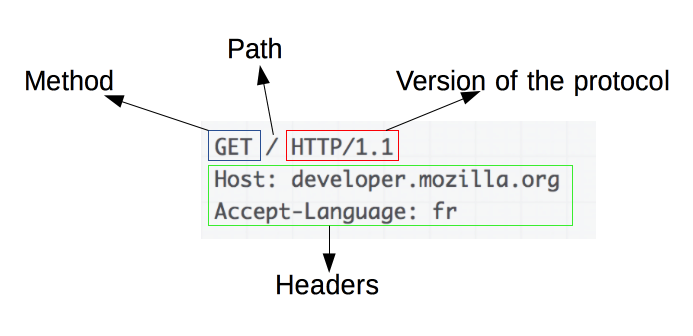
\includegraphics[width=0.5\textwidth,height=\textheight]{images/HTTP_Request.png}\\
\emph{Source :
\url{https://developer.mozilla.org/fr/docs/Web/HTTP/Aper\%C3\%A7u}}

\begin{enumerate}
\def\labelenumi{\arabic{enumi}.}
\item
  Avec un navigateur Web, demander la page d'adresse\\
  \url{http://frederic-junier.org/NSI/sandbox/index.html}.\\
  Ouvrir la barre d'outils de développement en appuyant sur la touche de
  fonction \passthrough{\lstinline!F12!} et sélectionner l'onglet
  Réseau. On peut voir les entêtes de la requête et de la réponse HTTP.

  \begin{itemize}
  \item
    Que représente le code d'état de la réponse HTTP ?

    \begin{quote}
    \emph{Réponse : Le code 200 indique que le serveur a pu envoyer la
    page demandée avec succès. On note qu'il s'agit d'une requête avec
    la méthode \url{GET}}
    \end{quote}

    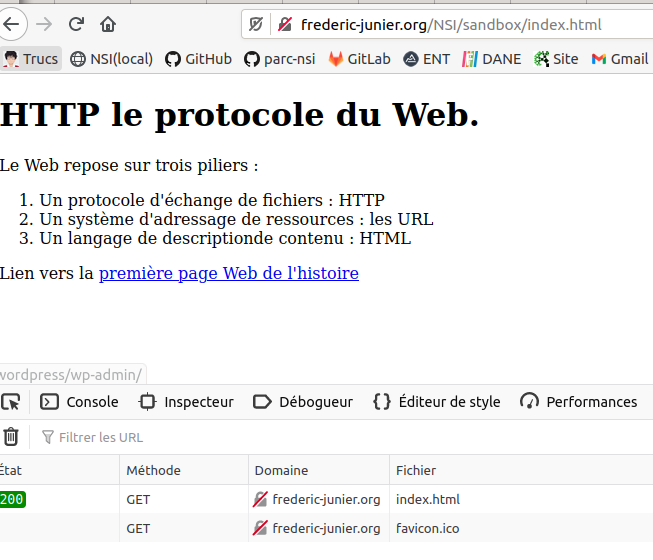
\includegraphics[width=0.5\textwidth,height=\textheight]{images/exo2_code_reponse_http.png}\\
  \item
    Quelles informations sur le client sont transmises au serveur dans
    l'entête de la requête ?

    \begin{quote}
    \emph{Réponse : Le client transmet plusieurs paramètres dans sa
    requête :} \emph{La méthode du protocole \url{HTTP} qui est
    utilisée, ici \url{GET} qui permet de demander une ressource}
    \emph{La version du protocole \url{HTTP} ici 1.1, c'est important de
    se mettre d'accord sur les règles du dialogue lorsqu'on communique
    !} \emph{\passthrough{\lstinline!Accept!} précise les types de
    contenus que le client pourra interpréter}
    \emph{\passthrough{\lstinline!Accept-Language!} précise la variante
    de la locale} \emph{\passthrough{\lstinline!Connection!} précise si
    le client souhaite une connexion persistante après l'échange
    requête/réponse avec le serveur : on garde la même connexion
    \url{TCP}} \emph{\passthrough{\lstinline!Cache-Control!} et
    \passthrough{\lstinline!If-Modified-Since!} contiennent des
    directives pour la mise en cache ou l'utilisation du cache du
    client} \emph{\passthrough{\lstinline!User-Agent!} contient
    différentes informations sur le navigateur et le système
    d'exploitation du client}
    \end{quote}
  \end{itemize}

  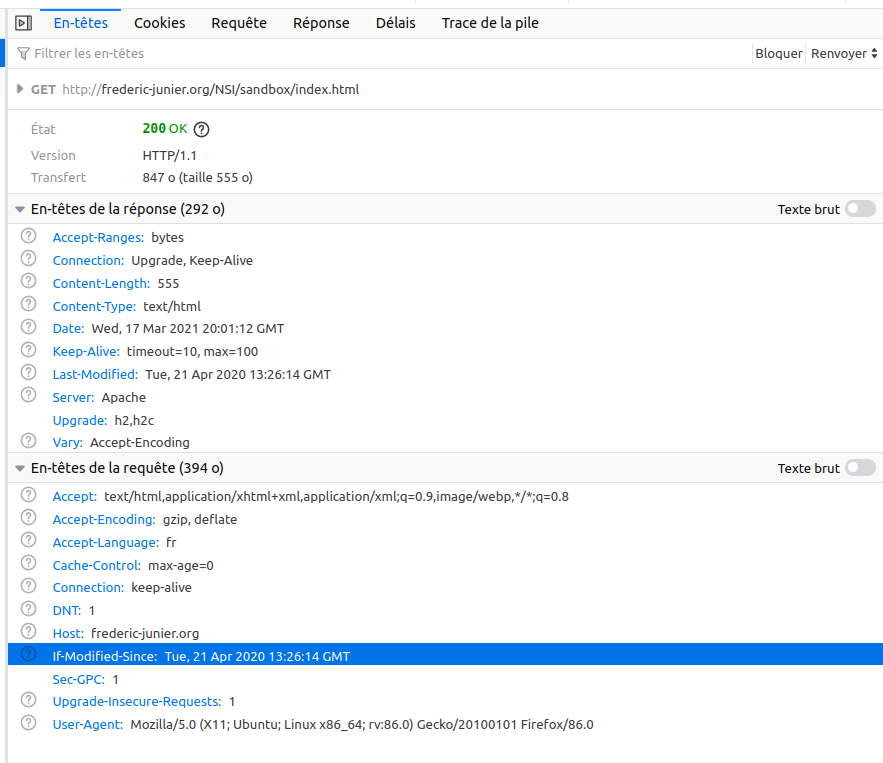
\includegraphics[width=1\textwidth,height=\textheight]{images/en_tete_http.png}\\

  \begin{itemize}
  \tightlist
  \item
    Quelles informations sur le serveur sont transmises au client dans
    l'entête de la réponse ?
  \end{itemize}

  \begin{quote}
  \emph{Réponse : Le serveur transmet plusieurs paramètres dans sa
  réponse :} \emph{\passthrough{\lstinline!Content-Length!} précise la
  taille en octets de la réponse}
  \emph{\passthrough{\lstinline!Content-Type!} précise le type de
  contenu de la réponse, ici du HTML}
  \emph{\passthrough{\lstinline!Date!} contient un horodatage de la
  réponse} \emph{\passthrough{\lstinline!Laste-Modified!} contient un
  horodatage de la dernière modification de la ressource}
  \emph{\passthrough{\lstinline!Server!} précise le type de logiciel
  serveur, ici \href{http://www.apache.org/}{Apache}}
  \end{quote}

  \begin{itemize}
  \tightlist
  \item
    Effectuer une nouvelle requête avec
    l'\href{https://developer.mozilla.org/fr/docs/Glossaire/URL}{URL}
    \url{http://frederic-junier.org/NSI/sandbox/}. Quelle différence
    avec la requête initiale ?
  \end{itemize}

  \begin{quote}
  \emph{Réponse : La page renvoyée est la même mais avec le code de
  réponse de redirection 304 Not Modified indique qu'il n'y a pas besoin
  de retransmettre les ressources demandées. C'est une redirection
  implicite vers une ressource mise en cache. Cela survient lorsque la
  méthode de requête est safe (par exemple une requête GET ou HEAD), ou
  lorsque la requête est conditionnelle et utilise l'en-tête
  If-None-Match ou If-Modified-Since. Noter que si le chemin de la
  ressource dans l'\url{URL} ne se termine pas par un fichier alors le
  serveur Web renvoie le fichier par défaut
  \passthrough{\lstinline!index.html!} s'il existe}
  \end{quote}

  \begin{itemize}
  \tightlist
  \item
    Effectuer une nouvelle requête avec
    l'\href{https://developer.mozilla.org/fr/docs/Glossaire/URL}{URL}
    \url{https://frederic-junier.org/NSI/sandbox/}. Quelle différence
    avec la requête initiale peut-on observer dans la barre d'adresse du
    navigateur ?
  \end{itemize}

  \begin{quote}
  \emph{Réponse : cette fois le petit cadenas n'est pas barré, la
  connexion est sécurisée : chiffrée en \url{HTTPS} et le serveur est
  authentifié par un certificat SSL à jour.}
  \end{quote}

  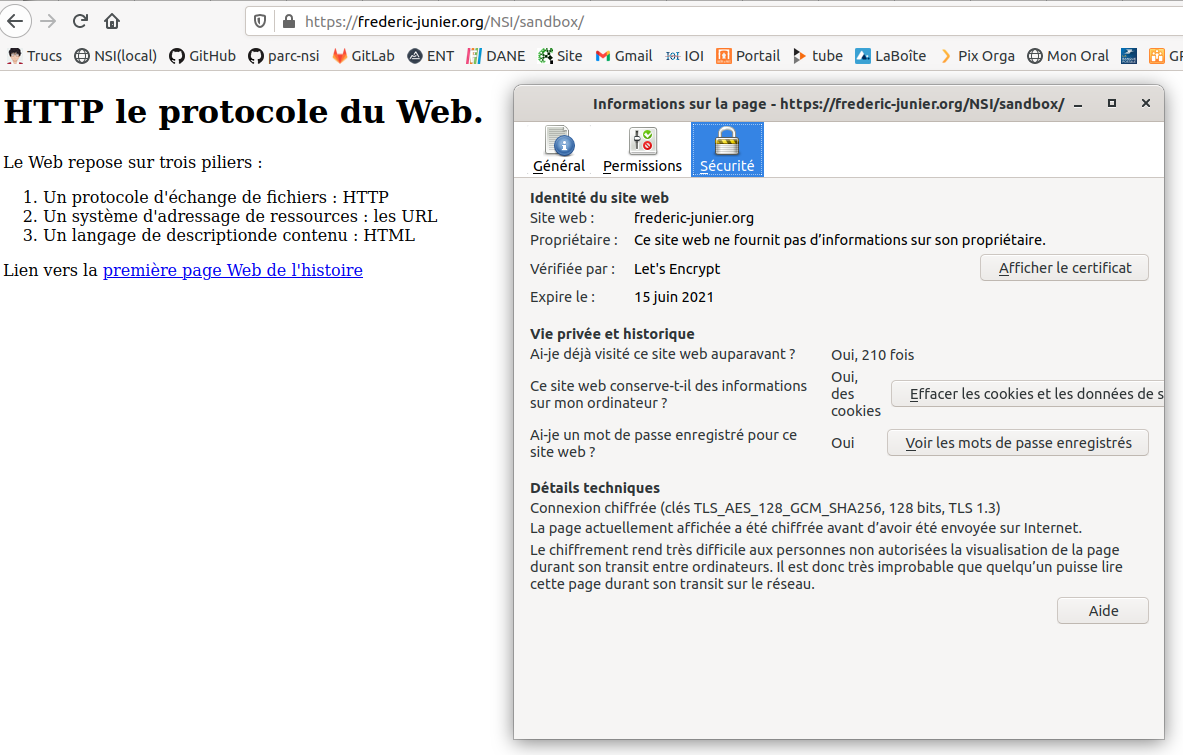
\includegraphics[width=0.8\textwidth,height=\textheight]{images/sandbox_https.png}\\

  \begin{itemize}
  \item
    Effectuer une nouvelle requête avec
    l'\href{https://developer.mozilla.org/fr/docs/Glossaire/URL}{URL}
    \url{http://frederic-junier.org/NSI/Sandbox/index.html}. Quel est le
    code d'état de la réponse ? Explication ?

    \begin{quote}
    \emph{Réponse : cette fois on a une erreur 404, c'est une erreur du
    client qui a demandé une ressource qui n'existe pas sur le serveur.
    Pourquoi ? C'est un problème de casse de caractère dans l'\url{URL}
    où il ne faut pas de majuscule sur sandbox.}
    \end{quote}
  \end{itemize}

  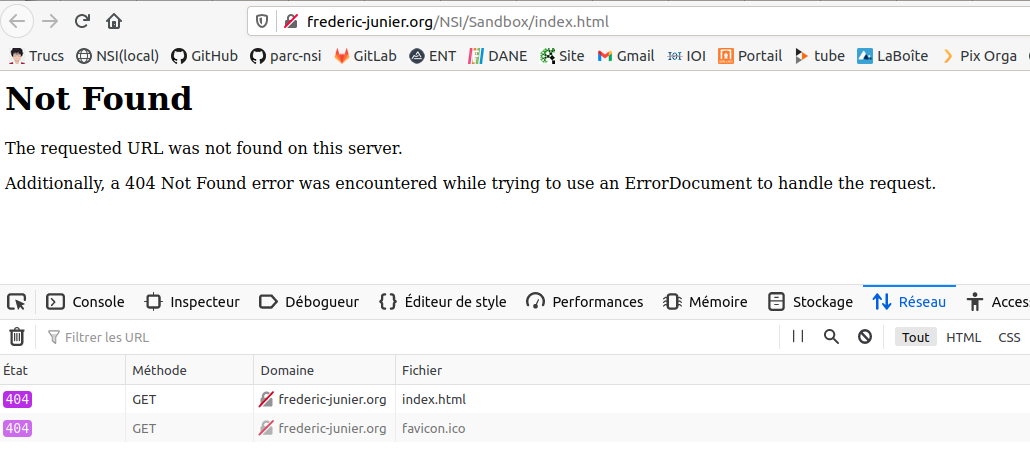
\includegraphics[width=0.8\textwidth,height=\textheight]{images/erreur_404.png}\\

  \begin{itemize}
  \tightlist
  \item
    Effectuer une nouvelle requête avec
    l'\href{https://developer.mozilla.org/fr/docs/Glossaire/URL}{URL}
    \url{http://frederic-junier.org/NSI/interdit}. Quel est le code
    d'état de la réponse ? Explication ?
  \end{itemize}

  \begin{quote}
  \emph{Réponse : cette fois on a une erreur 403 Forbidden : le serveur
  comprend la requête mais refuse de l'autoriser. En effet, les droits
  d'accès sur le répertoire interdit sont positionnés à 710 soit
  RWX--X---, donc aucun droit pour un utilisateur ``autre''}
  \end{quote}

  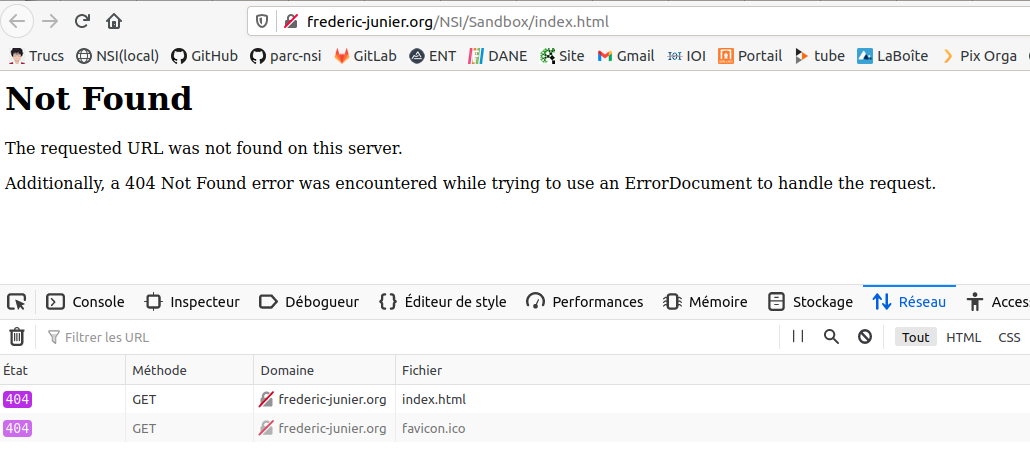
\includegraphics[width=0.8\textwidth,height=\textheight]{images/erreur_404.png}\\

  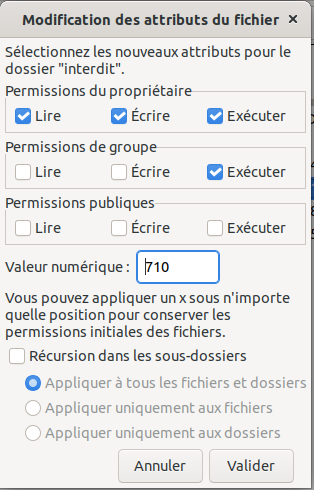
\includegraphics[width=0.5\textwidth,height=\textheight]{images/droits_interdit.png}\\
\item
  Le site \url{https://httpie.org/} propose un client HTTP en ligne de
  commandes permettant de décomposer les requêtes HTTP en précisant la
  méthode et l'URL de la ressource demandée.

  \begin{itemize}
  \tightlist
  \item
    Ouvrir la page \url{https://httpie.org/run}
  \item
    Saisir la commande
    \passthrough{\lstinline!http -v GET https://frederic-junier.org/NSI/sandbox/index.html!}.
    Décrire le fonctionnement de la méthode
    \passthrough{\lstinline!GET!} du protocole
    \passthrough{\lstinline!HTTP!} : formats de la requête et de la
    réponse.
  \end{itemize}

  \begin{quote}
  \emph{Réponse : la méthode \url{GET} du protocole \url{HTTP} est celle
  qui s'exécute par défaut lorsqu'on effectue une requête en saisissant
  l'\url{URL} de la page dans la barre d'adresse du navigateur. Voir
  ci-dessus pour les en-têtes client/serveur. On voit aussi apparaître
  le contenu de la réponse : le code source \url{HTML} de la page
  demandée.}
  \end{quote}

  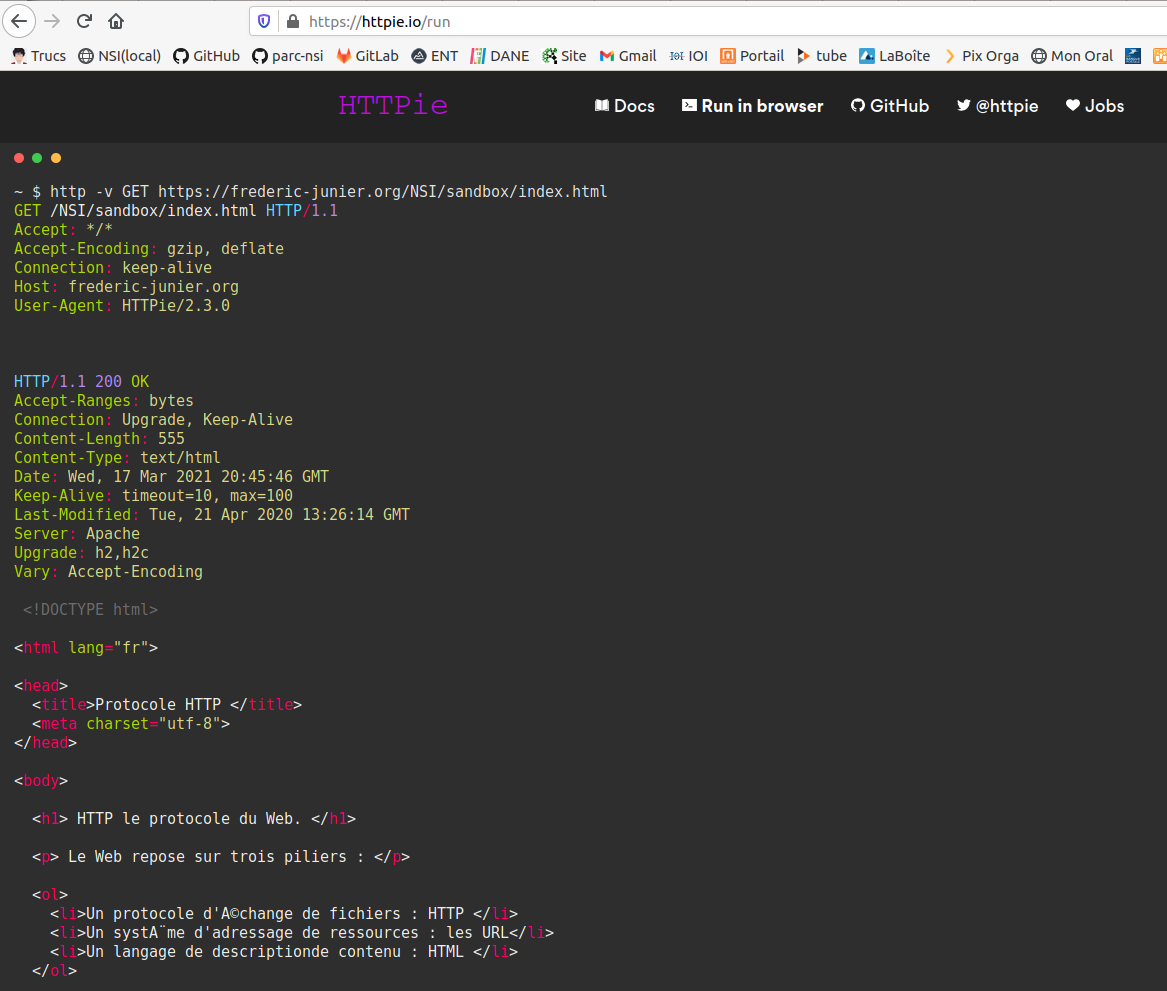
\includegraphics[width=0.8\textwidth,height=\textheight]{images/http_pie1.png}\\

  \begin{itemize}
  \tightlist
  \item
    Saisir la commande
    \passthrough{\lstinline!http -v HEAD https://frederic-junier.org/NSI/sandbox/index.html!}.
    Décrire le fonctionnement de la méthode
    \passthrough{\lstinline!HEAD!} du protocole
    \passthrough{\lstinline!HTTP!} : formats de la requête et de la
    réponse.
  \end{itemize}

  \begin{quote}
  \emph{Réponse : Avec la méthode \passthrough{\lstinline!HEAD!} on ne
  récupère que les en-têtes.}
  \end{quote}

  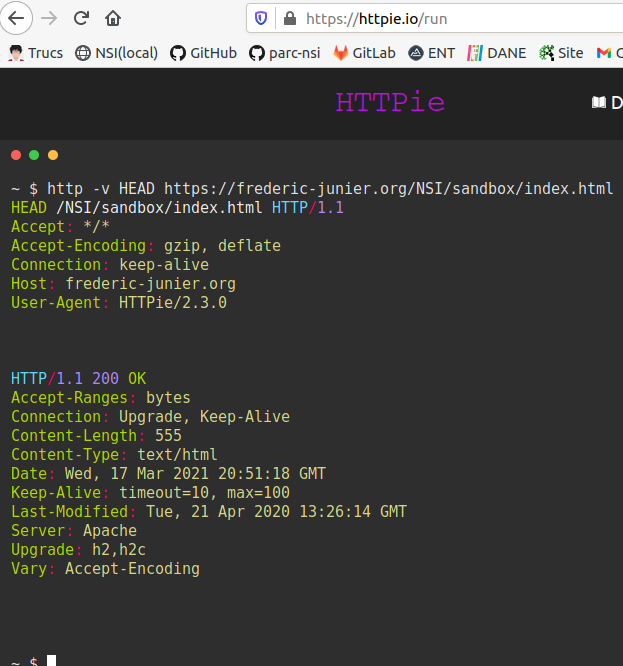
\includegraphics[width=0.8\textwidth,height=\textheight]{images/http_pie2.png}\\

  \begin{itemize}
  \tightlist
  \item
    Saisir la commande
    \passthrough{\lstinline!http -v PUT https://frederic-junier.org/NSI/sandbox/index.html hello=world!}.
    Quel résultat obtient-on ? Explication \footnote{Note : Méthodes
      HTTP : voir
      \url{https://developer.mozilla.org/fr/docs/Web/HTTP/M\%C3\%A9thode}}
    ?
  \end{itemize}

  \begin{quote}
  \emph{Réponse: La méthode PUT remplace toutes les représentations
  actuelles de la ressource visée par le contenu de la requête.Ici le
  serveur renvoie un code d'erreur 403 FORBIDDEN car un utilisateur
  ``autre'' ne peut pas modifier la ressource (heureusement).}
  \end{quote}
\end{enumerate}

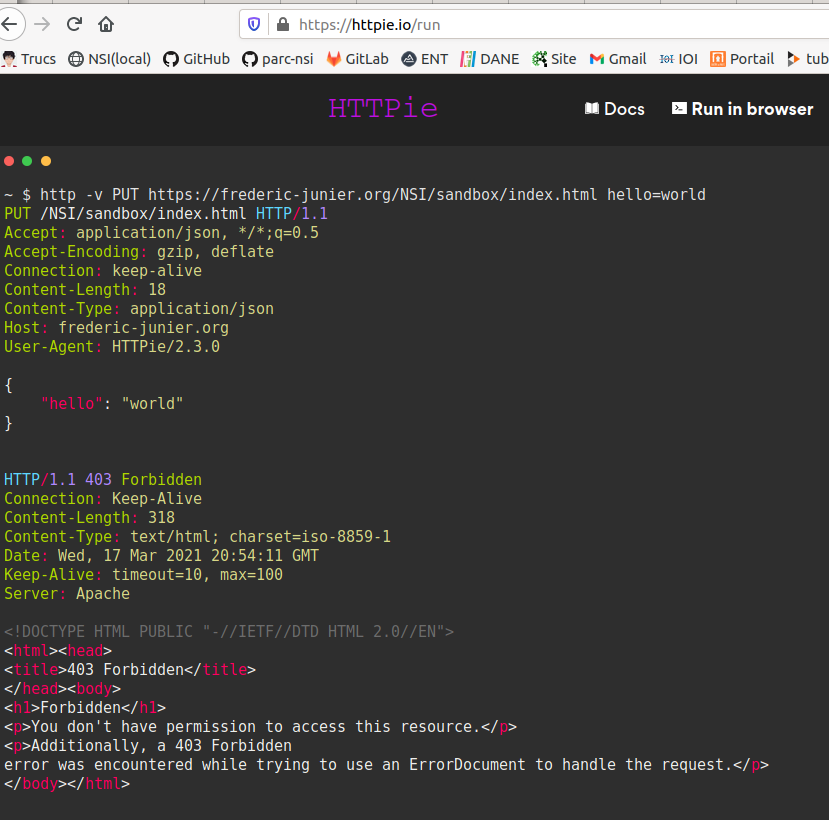
\includegraphics[width=0.8\textwidth,height=\textheight]{images/http_pie3.png}\\

\end{exercice}

\hypertarget{passage-de-paramuxe8tres-dans-une-url}{%
\subsection{Passage de paramètres dans une
URL}\label{passage-de-paramuxe8tres-dans-une-url}}

\begin{exercice}{}

Ouvrir un navigateur Web.

\begin{enumerate}
\def\labelenumi{\arabic{enumi}.}
\item
  Demander la page d'adresse
  \href{https://frederic-junier.org/NSI/sandbox/accueil.php}{http://frederic-junier.org/NSI/sandbox/accueil.php}

  Quel est l'affichage obtenu ?

  \begin{quote}
  \emph{Réponse : La requête est envoyée avec la méthode \url{GET}, le
  code 200 de la réponse du serveur indique un succès}
  \end{quote}

  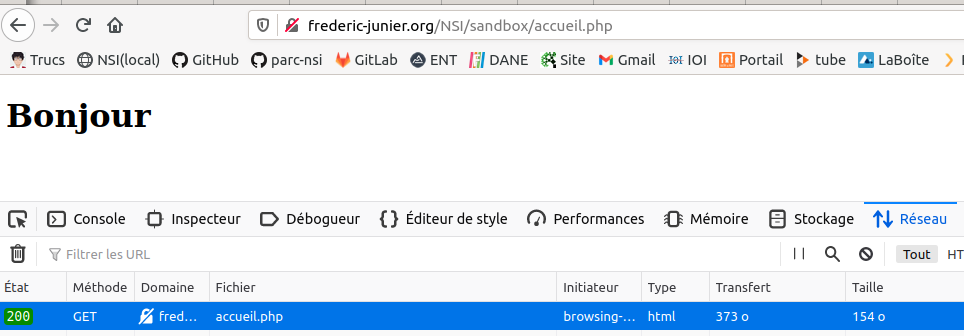
\includegraphics[width=0.8\textwidth,height=\textheight]{images/bonjour.png}\\
\item
  Demander la page d'adresse\\
  \href{https://frederic-junier.org/NSI/sandbox/accueil.php?nom=Turing\&prenom=Alan}{http://frederic-junier.org/NSI/sandbox/accueil.php?nom=Turing\&prenom=Alan}

  Quel est l'affichage obtenu ? Ouvrir les outils de développement avec
  \passthrough{\lstinline!F12!} puis sélectionner les onglets
  \passthrough{\lstinline!Réseau!} et
  \passthrough{\lstinline!Paramètres!}.

  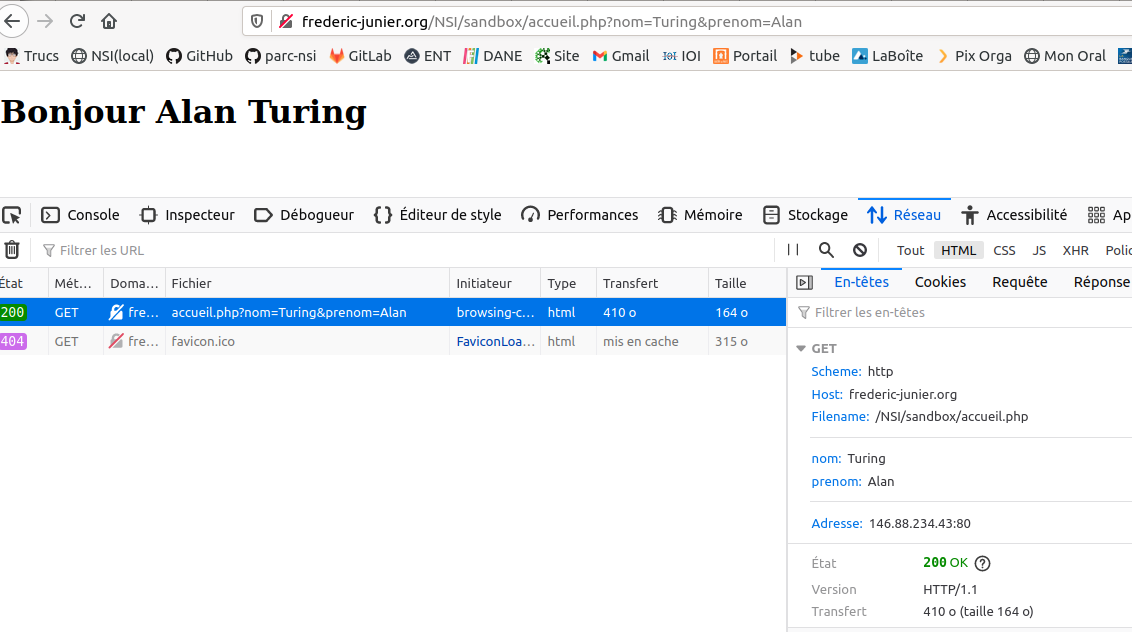
\includegraphics[width=0.8\textwidth,height=\textheight]{images/bonjour_get.png}\\
\end{enumerate}

\begin{quote}
\emph{Réponse : Dans la barre des outils de développement, onglet
Réseau, on a la décomposition de l'\url{URL} : le schéma (protocole http
), le nom de domaine (frederic-junier.org), le chemin vers la ressource
(/NSI/sandbox/accueil.php) et nouveauté des paramètres assemblés une
\textbf{chaîne de requête}, elle commence par le symbole
\passthrough{\lstinline!?!} puis contient une liste de paires
\passthrough{\lstinline!nom=valeur!} séparées par un symbole esperluette
\passthrough{\lstinline!\&!}. Ces paramètres ne font pas partie de
l'adresse de la ressource mais sont une façon pour le client de
transmettre des informations au serveur.}
\end{quote}

\begin{enumerate}
\def\labelenumi{\arabic{enumi}.}
\setcounter{enumi}{2}
\tightlist
\item
  Remplacer Turing par votre nom et Alan par votre prénom dans
  l'\href{https://developer.mozilla.org/fr/docs/Glossaire/URL}{URL}
  précédente. Que peut-on remarquer ? À votre avis, que se passe-t-il
  sur le serveur lorsqu'il reçoit la requête HTTP ?
\end{enumerate}

\begin{quote}
\emph{Réponse : côté serveur, un programme doit fabriquer la page
\url{HTML} renvoyée au client à la volée en fonction des paramètres
transmis. On parle dans ce cas de \textbf{page web dynamique}. Le
programme s'exécutant côté serveur est écrit en \url{PHP}. On donne le
code ci-dessous}
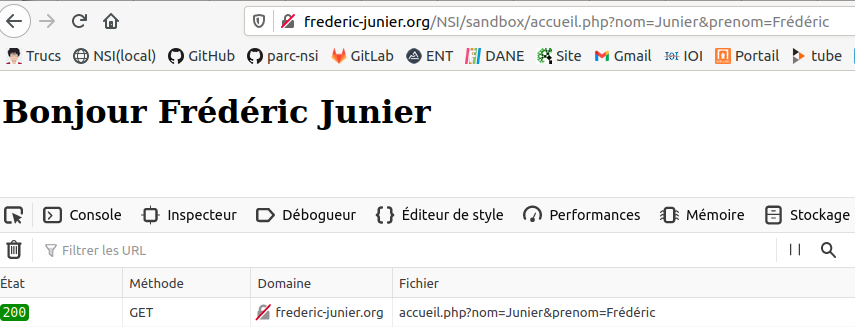
\includegraphics[width=0.8\textwidth,height=\textheight]{images/bonjour_frederic.png}\\
\end{quote}

\begin{enumerate}
\def\labelenumi{\arabic{enumi}.}
\setcounter{enumi}{3}
\tightlist
\item
  Voici le contenu du fichier \passthrough{\lstinline!accueil.php!} sur
  le serveur. S'agit-il d'un texte écrit en
  \href{https://developer.mozilla.org/fr/docs/Glossaire/HTML}{HTML} ?
  Faire une recherche sur la signification de l'acronyme
  \href{https://developer.mozilla.org/fr/docs/Glossaire/PHP}{PHP}.
\end{enumerate}

\begin{lstlisting}[language=PHP]
 <!DOCTYPE html>
<html lang="fr">
<head>
  <title>Accueil </title>
  <meta charset="utf-8">    
</head> 
<body>
<h1>
<?php  
echo "Bienvenue " . $_GET['prenom'] . " " .  $_GET['nom'] ;
?>
</h1>
</body>
</html> 
\end{lstlisting}

\begin{enumerate}
\def\labelenumi{\arabic{enumi}.}
\setcounter{enumi}{3}
\tightlist
\item
  Enregistrer
  l'\href{https://developer.mozilla.org/fr/docs/Glossaire/URL}{URL}
  testée précédemment dans les marque-pages du navigateur. Ouvrir un
  autre onglet et cliquer sur le signet enregistré. Retrouve-t-on la
  même page Web ?
\end{enumerate}

\begin{quote}
\emph{Réponse : il est tout à fait possible d'enregistrer une
\href{https://developer.mozilla.org/fr/docs/Glossaire/URL}{URL} avec
paramètres dans les signets de son navigateur.}
\end{quote}

\end{exercice}

\hypertarget{formulaire-et-passage-de-paramuxe8tres}{%
\section{Formulaire et passage de
paramètres}\label{formulaire-et-passage-de-paramuxe8tres}}

\hypertarget{un-premier-exemple}{%
\subsection{Un premier exemple}\label{un-premier-exemple}}

\begin{exemple}{}

\begin{enumerate}
\def\labelenumi{\arabic{enumi}.}
\item
  Ouvrir avec un navigateur Web la page
  d'\href{https://developer.mozilla.org/fr/docs/Glossaire/URL}{URL} :

  \url{http://frederic-junier.org/NSI/sandbox/formulaire-get.html}

  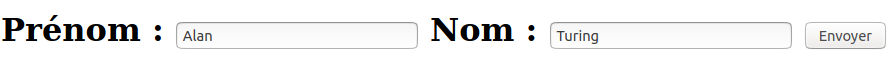
\includegraphics{images/formulaire1.png}\\

  \begin{itemize}
  \tightlist
  \item
    Cliquer sur le bouton \passthrough{\lstinline!Envoyer!}. Que se
    passe-t-il ? Rafraîchir la page avec \passthrough{\lstinline!F5!}.
    Que se passe-t-il ?
  \end{itemize}

  \begin{quote}
  \emph{Réponse : en cliquant sur le bouton envoyer, on génère côté
  client une \url{URL} avec comme paramètres les valeurs des champs du
  formulaire :
  \url{http://frederic-junier.org/NSI/sandbox/accueil.php?prenom=Alan\&nom=Turing}.
  Le client envoie au serveur sa requête avec la méthode \url{GET} Si on
  rafraichit la page avec F5, le comportement est répété à l'identique
  puisque le client construit la même requête à partir de l'\url{URL}
  avec paramètres.}
  \end{quote}

  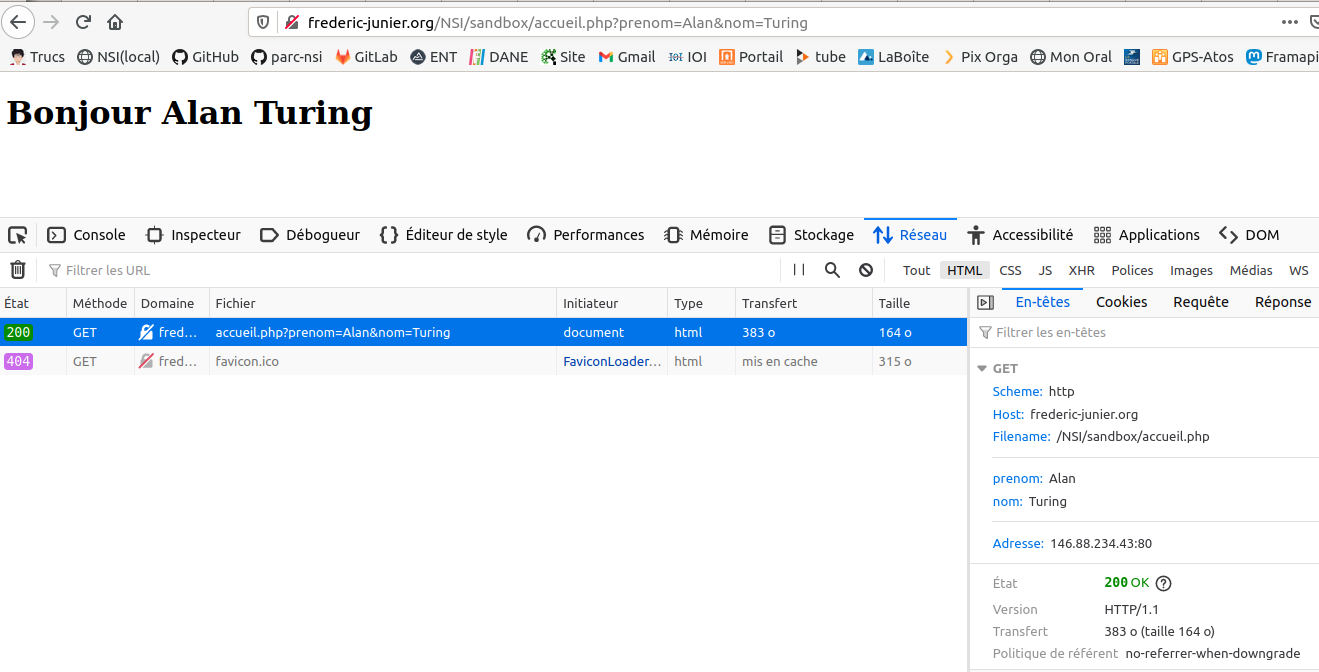
\includegraphics{images/requete_formulaire.png}\\

  \begin{itemize}
  \tightlist
  \item
    Changer les valeurs des champs \passthrough{\lstinline!Prénom!} et
    \passthrough{\lstinline!Nom!} du formulaire puis cliquer sur le
    bouton \passthrough{\lstinline!Envoyer!}. Que se passe-t-il ?
  \end{itemize}

  \begin{quote}
  \emph{Réponse : mise à jour, une partie de la logique pour générer la
  page web dynamique est déportée côté client (choix des paramètres dans
  une \href{}{Interaction Homme
  Machine}https://interstices.info/domaine/interaction-hommemachine/
  représentée par le formulaire). Noter que les paramètres apparaissent
  dans l'onglet en-tête \url{GET} des outils de développement et non
  dans l'onglet Requête}.
  \end{quote}

  \begin{itemize}
  \tightlist
  \item
    Ouvrir la fenêtre des outils de développement et afficher dans
    l'onglet Réseau l'entête de la requête HTTP qui devrait ressembler à
    celui-ci :
  \end{itemize}

  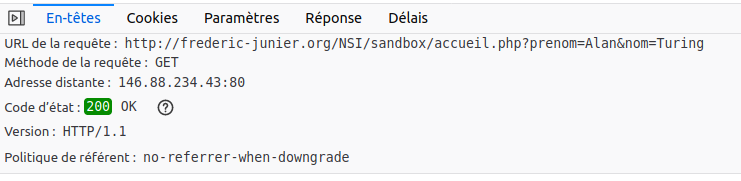
\includegraphics[width=0.8\textwidth,height=\textheight]{images/entete-get.png}\\

  Sélectionner l'onglet Paramètres et vérifier qu'on obtient les
  paramètres transmis à travers
  l'\href{https://developer.mozilla.org/fr/docs/Glossaire/URL}{URL} dans
  la chaîne de requête comme dans l'exercice 3.

  \begin{itemize}
  \tightlist
  \item
    Afficher le code source de la page
    \passthrough{\lstinline!formulaire-get.html!} avec le raccourci
    clavier \passthrough{\lstinline!CRTL + U!}. On devrait obtenir le
    texte ci-dessous :
  \end{itemize}

\begin{lstlisting}[language=HTML]
<!DOCTYPE html>

<html lang="fr">

<head>
<title>Formulaire HTML </title>
<meta charset="utf-8">    
</head> 
<body>

   <form action = "accueil.php" method="GET">        
      <label for="id_prenom">Prénom :</label>
      <input type="text" id="id_prenom" name="prenom" value="Alan">
      <label for="id_nom">Nom :</label>
      <input type="text" id="id_nom" name="nom" value="Turing">
      <button type="submit" id="bouton">Envoyer</button>
   </form>

</body>
</html> 
\end{lstlisting}
\item
  Ouvrir avec un navigateur Web la page
  d'\href{https://developer.mozilla.org/fr/docs/Glossaire/URL}{URL} :

  \url{http://frederic-junier.org/NSI/sandbox/formulaire-post.html}

  \begin{itemize}
  \tightlist
  \item
    Cliquer sur le bouton \passthrough{\lstinline!Envoyer!}. Que se
    passe-t-il ?
  \end{itemize}

  \begin{quote}
  \emph{Réponse : le serveur renvoie la même page que pour la requête
  précédente mais cette fois les paramètres du formulaire ne sont pas
  transmis à travers l'\url{URL} et donc dans l'entête \url{HTTP} comme
  avec la méthode \url{GET}. Ils sont transmis dans le corps de la
  requête \url{HTTP} comme on peut le voir dans l'onglet Requête des
  outils de développement. On peut remarquer que la méthode de la
  requête \url{HTTP} a changé, il s'agit de la méthode \url{POST}}.
  \end{quote}

  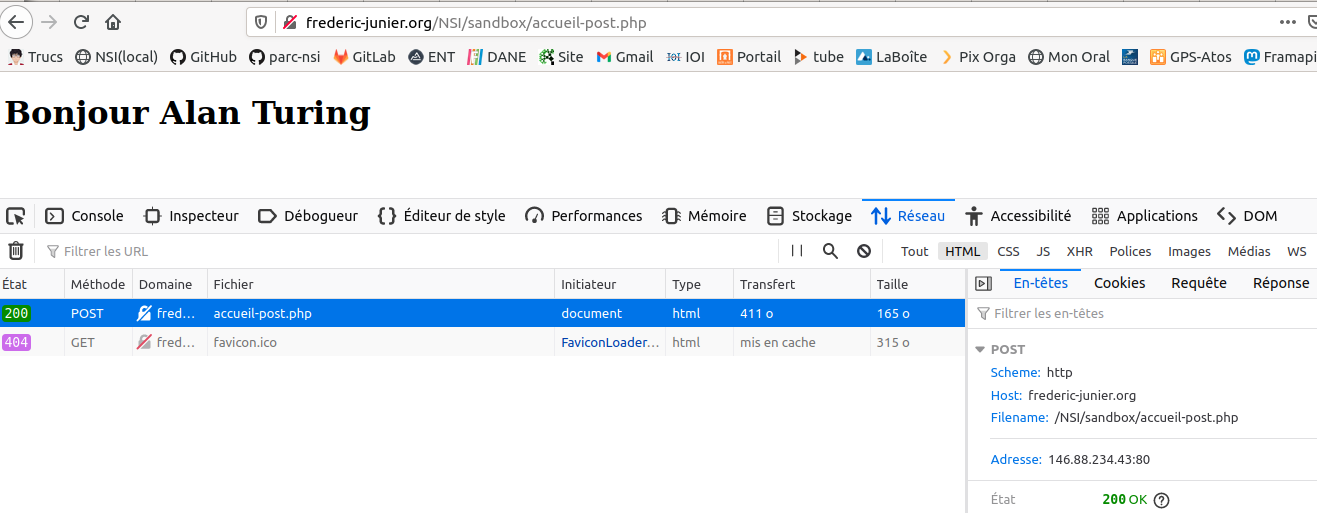
\includegraphics[width=0.8\textwidth,height=\textheight]{images/requete_formulaire_post.png}\\

  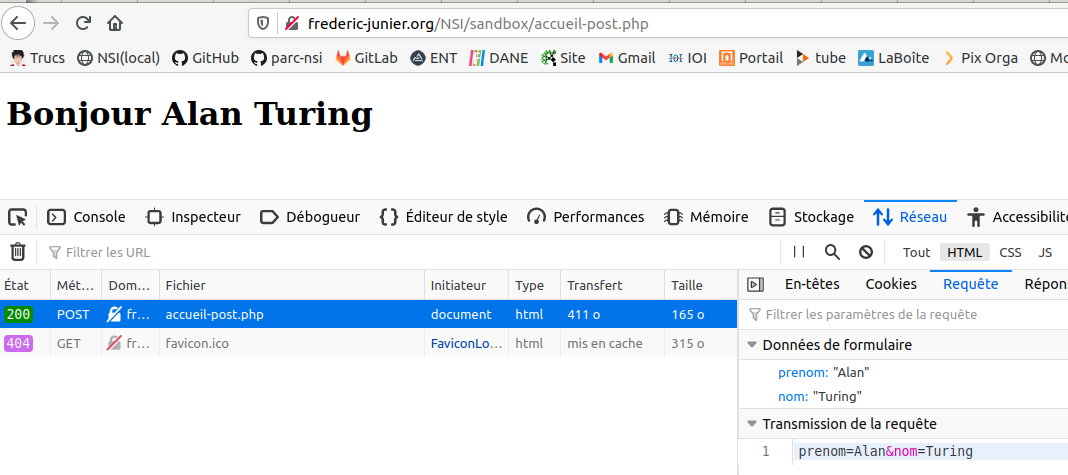
\includegraphics[width=0.8\textwidth,height=\textheight]{images/requete_formulaire_post2.png}\\

  \begin{itemize}
  \tightlist
  \item
    Changer les valeurs des champs \passthrough{\lstinline!Prénom!} et
    \passthrough{\lstinline!Nom!} du formulaire puis cliquer sur le
    bouton \passthrough{\lstinline!Envoyer!}. Que se passe-t-il ?
    Observe-t-on un changement dans
    l'\href{https://developer.mozilla.org/fr/docs/Glossaire/URL}{URL} de
    la requête ? dans son entête ?
  \end{itemize}

  \begin{quote}
  \emph{Réponse :comme on l'a écrit ci-dessus, la méthode \url{POST}
  n'envoie pas les paramètres de formulaire à travers l'\url{URL} et
  l'entête \url{HTTP} comme avec la méthode \url{GET} mais directement
  dans le corps de la requête}.
  \end{quote}

  \begin{itemize}
  \item
    Rafraîchir la page avec \passthrough{\lstinline!F5!}. Que se
    passe-t-il ?

    \begin{quote}
    \emph{Réponse : \url{HTTP} est un protocole sans mémoire, pour
    générer la page web il faut renvoyer les paramètres qui ne sont pas
    dans l'\url{URL} d'où l'avertissement ci-dessous.}
    \end{quote}
  \end{itemize}

  
\includegraphics[width=0.7\textwidth,height=\textheight]{images/avertissement-post.png}\\

  \begin{itemize}
  \tightlist
  \item
    Ouvrir la fenêtre des outils de développement et afficher dans
    l'onglet Réseau l'entête de la requête HTTP qui devrait ressembler à
    celui-ci :
  \end{itemize}

  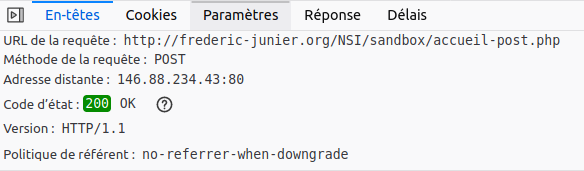
\includegraphics[width=0.6\textwidth,height=\textheight]{images/entete-post.png}\\

  Sélectionner l'onglet Paramètres et vérifier qu'on retrouve les
  paramètres transmis dans
  l'\href{https://developer.mozilla.org/fr/docs/Glossaire/URL}{URL}.
  Quelle différence par rapport à la méthode vue en question 1 ?

  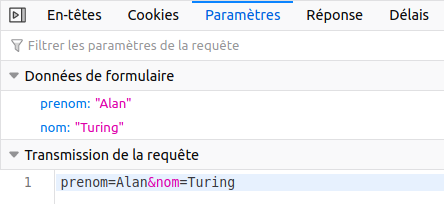
\includegraphics[width=0.4\textwidth,height=\textheight]{images/parametres2.png}\\

  \begin{itemize}
  \tightlist
  \item
    Afficher le code source de la page
    \passthrough{\lstinline!formulaire-post.html!} avec le raccourci
    clavier \passthrough{\lstinline!CRTL + U!}. Quels sont les deux
    changements par rapport au code de
    \passthrough{\lstinline!formulaire-get.html!} ?
  \end{itemize}

  \begin{quote}
  \_Réponse :
  \end{quote}
\end{enumerate}

\begin{lstlisting}[language=HTML]
 <!DOCTYPE html>

<html lang="fr">

<head>
  <title>Formulaire HTML </title>
  <meta charset="utf-8">    
</head>
 
<body>

    <!-- Changement dans la balise form par rapport à formulaire-get.html : la cible et la méthode  -->
    <form action = "accueil-post.php" method="post">
        
        <label for="id_prenom">Prénom :</label>
        <input type="text" id="id_prenom" name="prenom" value="Alan">

        <label for="id_nom">Nom :</label>
        <input type="text" id="id_nom" name="nom" value="Turing">

        <button type="submit" id="bouton">Envoyer</button>

    </form>


</body>
</html> 
\end{lstlisting}

\end{exemple}

\hypertarget{muxe9thodes-de-passage-des-paramuxe8tres-get-ou-post}{%
\subsection{Méthodes de passage des paramètres : GET ou
POST}\label{muxe9thodes-de-passage-des-paramuxe8tres-get-ou-post}}

\begin{exercice}{}

\emph{QCM} de type E3C2.

\begin{enumerate}
\def\labelenumi{\arabic{enumi}.}
\item
  Parmi les réponses suivantes, que permet d'effectuer la méthode
  \href{https://developer.mozilla.org/fr/docs/Web/HTTP/M\%C3\%A9thode/POST}{POST}
  du protocole
  \href{https://developer.mozilla.org/fr/docs/Glossaire/HTTP}{HTTP}~?

  \begin{itemize}
  \tightlist
  \item
    Réponse A : Définir le style d'une page web
  \item
    Réponse B : Pirater des données bancaire\\
  \item
    Réponse C : Envoyer une page web vers le client\\
  \item
    Réponse D : Envoyer les données saisies dans un formulaire HTML vers
    un serveur \textbf{=\textgreater{} BONNE RÉPONSE}
  \end{itemize}
\item
  Un site internet utilise une requête
  \href{https://developer.mozilla.org/fr/docs/Glossaire/HTTP}{HTTP} avec
  la méthode
  \href{https://developer.mozilla.org/fr/docs/Web/HTTP/M\%C3\%A9thode/POST}{POST}
  pour transmettre les données d'un formulaire. Laquelle des
  affirmations suivantes est \textbf{incorrecte}~?

  \begin{itemize}
  \tightlist
  \item
    Réponse A : les données envoyées ne sont pas visibles
    \textbf{=\textgreater{} BONNE RÉPONSE}
  \item
    Réponse B : il est possible de transmettre des données de type
    binaire
  \item
    Réponse C : les données transmises sont cryptées
  \item
    Réponse D : il n'y a pas de restriction de longueur pour les données
    transmises
  \end{itemize}
\item
  Un internaute clique sur un lien qui envoie la requête
  \href{https://developer.mozilla.org/fr/docs/Glossaire/HTTP}{HTTP}
  suivante à un serveur~:

  \passthrough{\lstinline!http://jaimelaneige.com/ma\_planche/traitement.php?nom=Snow\&prenom=Jon!}

  Que demande cette requête au serveur ?

  \begin{itemize}
  \tightlist
  \item
    Réponse A : de renvoyer le fichier traitement.php en identifiant nom
    et prénom à Snow et Jon
  \item
    Réponse B : d'exécuter le fichier traitement.php en identifiant nom
    et prénom à Snow et Jon \textbf{=\textgreater{} BONNE RÉPONSE}
  \item
    Réponse C : d'indiquer si Jon Snow a bien pris son traitement
  \item
    Réponse D : de renvoyer le fichier traitement.php en affichant
    prénom et nom : Jon
  \end{itemize}
\end{enumerate}

\end{exercice}

\hypertarget{eluxe9ments-de-formulaire}{%
\subsection{Eléments de formulaire}\label{eluxe9ments-de-formulaire}}

\begin{exercice}{}

\begin{enumerate}
\def\labelenumi{\arabic{enumi}.}
\tightlist
\item
  Ouvrir dans un navigateur Web la page dont
  l'\href{https://developer.mozilla.org/fr/docs/Glossaire/URL}{URL} est
  :\\
  \url{https://repl.it/@fredericjunier/NSI-formulaire-exo5-radio}.

  \begin{itemize}
  \tightlist
  \item
    Cliquer sur \passthrough{\lstinline!Run!} pour lancer le serveur,
    remplir le formulaire contenu dans le fichier
    \passthrough{\lstinline!index.php!} et envoyer les données. Quelle
    méthode est utilisée pour le passage des paramètres du formulaire ?
  \end{itemize}
\end{enumerate}

\begin{quote}
\emph{Réponse : Les paramètres du formulaire sont transmis avec la
méthode \url{POST} }
\end{quote}

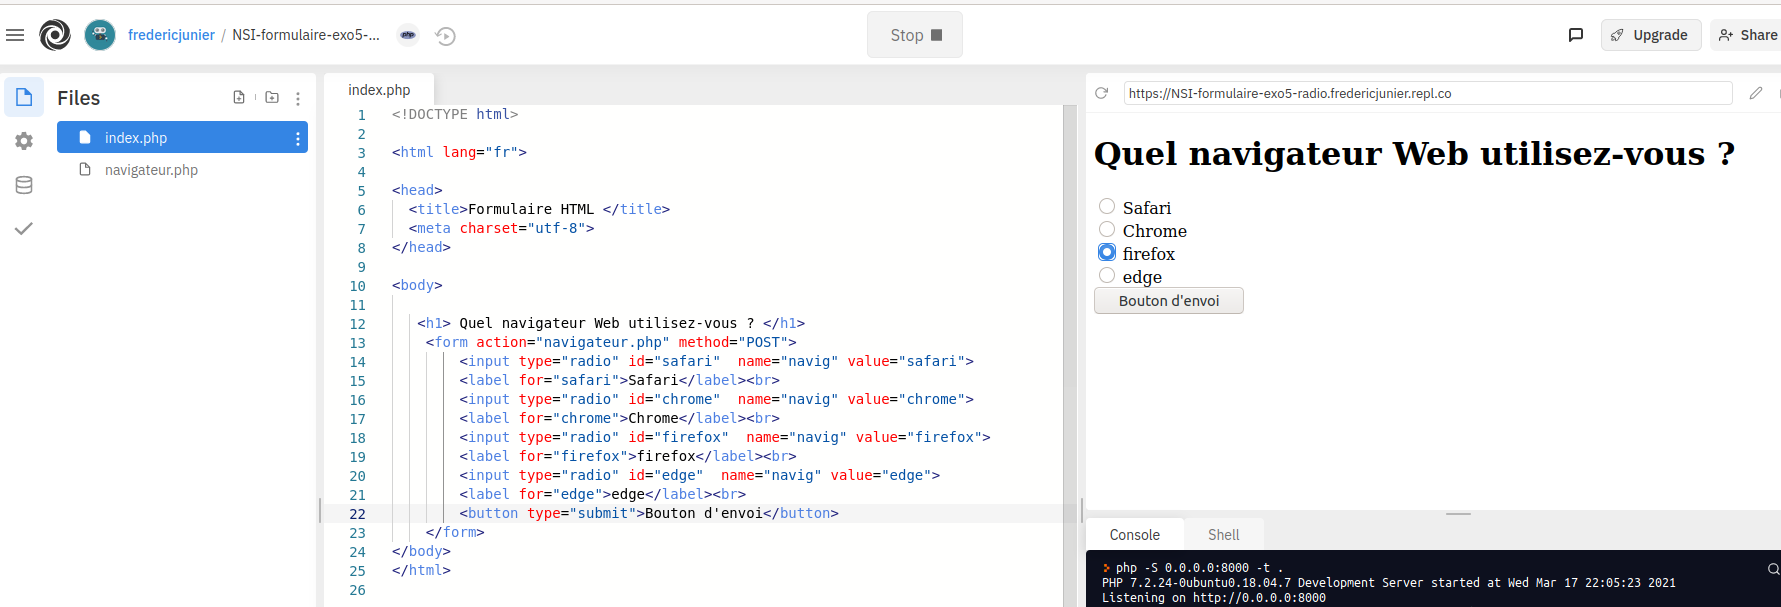
\includegraphics{images/formulaire_replit.png}\\

\begin{itemize}
\tightlist
\item
  Modifier les codes sources des fichiers
  \passthrough{\lstinline!index.php!} et
  \passthrough{\lstinline!navigateur.php!} pour changer la méthode de
  passage des paramètres du formulaire. En
  \href{https://developer.mozilla.org/fr/docs/Glossaire/PHP}{PHP}, on
  récupère la valeur du paramètre \passthrough{\lstinline!nom!} avec
  \passthrough{\lstinline!$\_GET['nom']!} si la méthode est
  \href{https://developer.mozilla.org/fr/docs/Web/HTTP/M\%C3\%A9thode/GET}{GET}
  ou \passthrough{\lstinline!$\_POST['nom']!} si c'est
  \href{https://developer.mozilla.org/fr/docs/Web/HTTP/M\%C3\%A9thode/POST}{POST}.
\end{itemize}

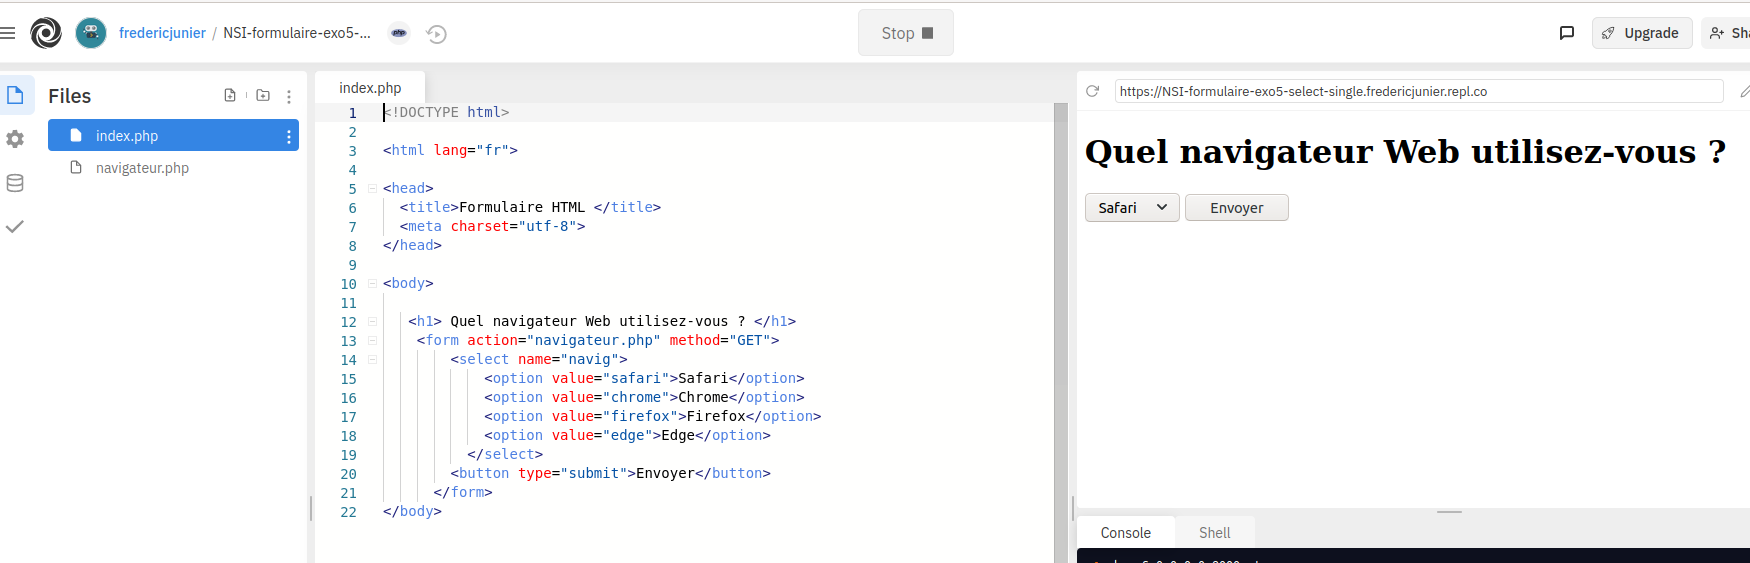
\includegraphics{images/formulaire_replit_select.png}\\

\begin{quote}
\emph{Réponse : code source modifié du fichier qui contient le
formulaire \passthrough{\lstinline!index.php!}}
\end{quote}

\begin{lstlisting}[language=PHP]
<!DOCTYPE html>

<html lang="fr">

<head>
  <title>Formulaire HTML </title>
  <meta charset="utf-8">    
</head>
 
<body>

   <h1> Quel navigateur Web utilisez-vous ? </h1>
    <form action="navigateur.php" method="GET">
        <select name="navig">
            <option value="safari">Safari</option>
            <option value="chrome">Chrome</option>
            <option value="firefox">Firefox</option>
            <option value="edge">Edge</option>
          </select> 
        <button type="submit">Envoyer</button>
      </form> 
</body>
\end{lstlisting}

\begin{quote}
\emph{Réponse : code source modifié du fichier qui génère la page à
partir des données du formulaire
\passthrough{\lstinline!navigateur.php!}}
\end{quote}

\begin{lstlisting}[language=PHP]
<!DOCTYPE html>

<html lang="fr">

<head>
  <title>Accueil </title>
  <meta charset="utf-8">    
</head>
 
<body>

<h1>
<?php  
echo "Vous utilisez le navigateur " . $_GET['navig'] ;
?>
</h1>

<a href="index.php">Retour au formulaire</a>
</body>
</html> 
\end{lstlisting}

\begin{itemize}
\tightlist
\item
  Consulter la documentation sur l'élément de formulaire
  \passthrough{\lstinline!<select>!} contenue dans la page
  \url{https://www.w3schools.com/html/html_form_elements.asp} et
  remplacer les \passthrough{\lstinline!<input>!} de type
  \passthrough{\lstinline!radio!} du formulaire dans
  \passthrough{\lstinline!index.php!} par un élément
  \passthrough{\lstinline!<select>!} avec choix unique.
\end{itemize}

\begin{enumerate}
\def\labelenumi{\arabic{enumi}.}
\setcounter{enumi}{1}
\tightlist
\item
  Ouvrir dans un navigateur Web la page dont
  l'\href{https://developer.mozilla.org/fr/docs/Glossaire/URL}{URL} est
  :\\
  \url{https://repl.it/@fredericjunier/NSI-formulaire-exo5-checkbox}.

  \begin{itemize}
  \tightlist
  \item
    Cliquer sur \passthrough{\lstinline!Run!} pour lancer le serveur,
    remplir le formulaire contenu dans le fichier
    \passthrough{\lstinline!index.php!} et envoyer les données. Quelle
    méthode est utilisée pour le passage des paramètres du formulaire ?
  \end{itemize}

  \begin{quote}
  \emph{Réponse : les paramètres de formulaire sont envoyés avec la
  méthode \url{GET}}
  \end{quote}
\end{enumerate}

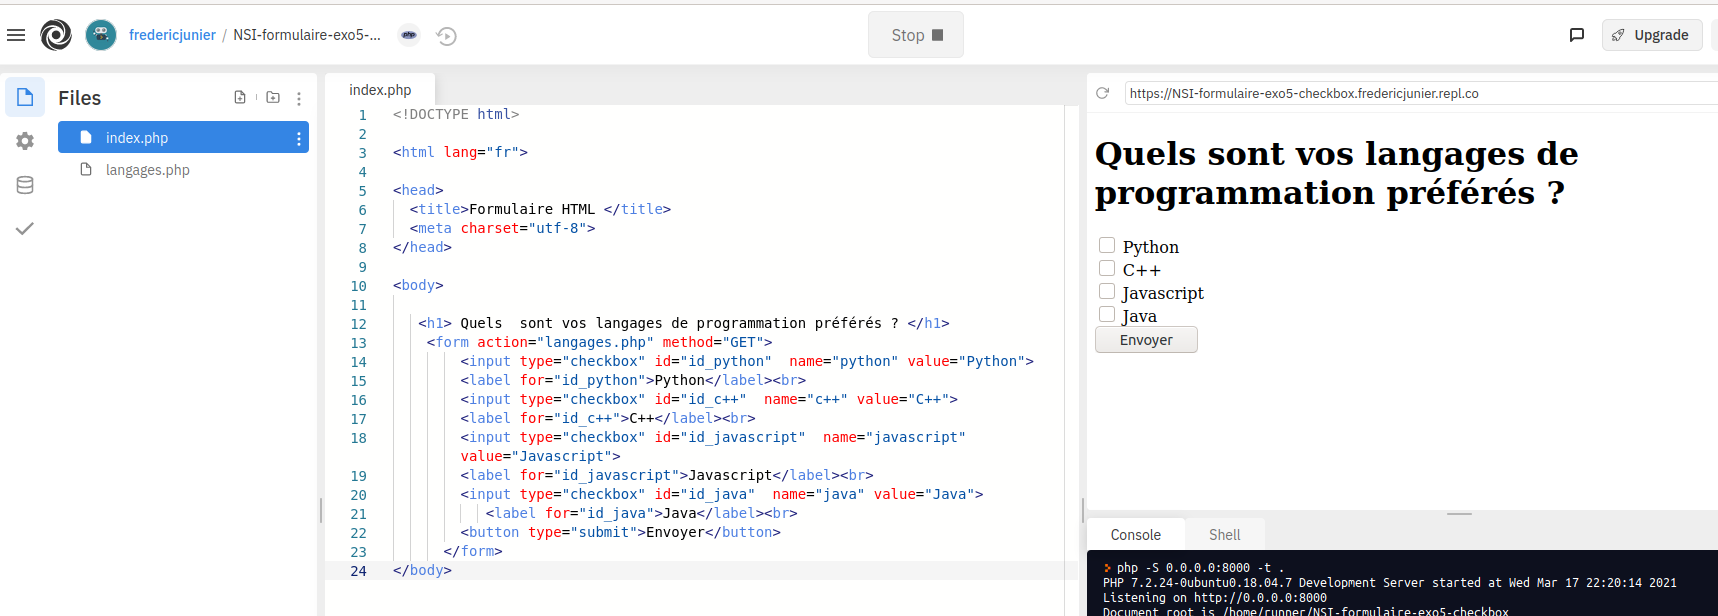
\includegraphics{images/formulaire_replit_checkbox.png}\\

\begin{itemize}
\tightlist
\item
  Modifier les codes sources des fichiers
  \passthrough{\lstinline!index.php!} et
  \passthrough{\lstinline!langages.php!} pour changer la méthode de
  passage des paramètres du formulaire.
\end{itemize}

\begin{quote}
\emph{Réponse : code de \passthrough{\lstinline!index.php!} pour
utiliser la méthode \url{POST}}
\end{quote}

\begin{lstlisting}[language=PHP]
<!DOCTYPE html>

<html lang="fr">

<head>
  <title>Formulaire HTML </title>
  <meta charset="utf-8">    
</head>
 
<body>

   <h1> Quels  sont vos langages de programmation préférés ? </h1>
    <form action="langages.php" method="POST">
        <input type="checkbox" id="id_python"  name="python" value="Python">
        <label for="id_python">Python</label><br>
        <input type="checkbox" id="id_c++"  name="c++" value="C++">
        <label for="id_c++">C++</label><br>
        <input type="checkbox" id="id_javascript"  name="javascript" value="Javascript">
        <label for="id_javascript">Javascript</label><br>
        <input type="checkbox" id="id_java"  name="java" value="Java">
           <label for="id_java">Java</label><br>
        <button type="submit">Envoyer</button>
      </form> 
</body>
\end{lstlisting}

\begin{quote}
\emph{Réponse : code de \passthrough{\lstinline!langages.php!} pour
utiliser la méthode \url{POST}}
\end{quote}

\begin{lstlisting}[language=PHP]
<!DOCTYPE html>

<html lang="fr">

<head>
  <title>Accueil </title>
  <meta charset="utf-8">    
</head>
 
<body>

<p>
   Vos langages préférés sont :
</p>
<ul>
<?php  
foreach ($_POST as $_langage) {
    echo "<li>" . $_langage . "</li>";
}
?>
</ul>


</body>
</html> 
\end{lstlisting}

\begin{itemize}
\tightlist
\item
  Consulter la documentation sur l'élément de formulaire
  \passthrough{\lstinline!<select>!} contenue dans la page
  \url{https://www.w3schools.com/html/html_form_elements.asp} et
  remplacer les \passthrough{\lstinline!<input>!} de type
  \passthrough{\lstinline!checkbox!} du formulaire dans
  \passthrough{\lstinline!index.php!} par un élément
  \passthrough{\lstinline!<select>!} avec choix multiple. Pour modifier
  le code \url{PHP} on s'inspirera de ce
  \href{https://stackoverflow.com/questions/2407284/how-to-get-multiple-selected-values-of-select-box-in-php/2407401\#2407401}{post
  stackoverflow}.
\end{itemize}

\begin{quote}
\emph{Réponse : code de \passthrough{\lstinline!index.php!} pour
utiliser un formulaire \passthrough{\lstinline!<select>!} multiple}
\end{quote}

\begin{lstlisting}[language=PHP]
<!DOCTYPE html>

<html lang="fr">

<head>
  <title>Formulaire HTML </title>
  <meta charset="utf-8">    
</head>
 
<body>

   <h1> Quels  sont vos langages de programmation préférés ? </h1>
    <form action="langages.php" method="GET">
      <select  id="top_langages" name="top_langages[]" multiple>
        <option value="Python">
        <label for="id_python">Python</label><br>
       <option value="c++">
        <label for="id_c++">C++</label><br>
        <option value="javascript">
        <label for="id_javascript">Javascript</label><br>
        <option value="java">
           <label for="id_java">Java</label><br>
      </select>
        <button type="submit">Envoyer</button>
      </form> 
</body>
\end{lstlisting}

\begin{quote}
\emph{Réponse : code de \passthrough{\lstinline!langages.php!} pour
utiliser un formulaire \passthrough{\lstinline!<select>!} multiple}
\end{quote}

\begin{lstlisting}[language=PHP]
<!DOCTYPE html>

<html lang="fr">

<head>
  <title>Accueil </title>
  <meta charset="utf-8">    
</head>
 
<body>

<p>
   Vos langages préférés sont :
</p>
<ul>
<?php 
foreach ($_GET["top_langages"] as $_langage) {
    echo "<li>" . $_langage . "</li>";
}
?>
</ul>


</body>
</html> 
\end{lstlisting}

\begin{enumerate}
\def\labelenumi{\arabic{enumi}.}
\setcounter{enumi}{3}
\tightlist
\item
  Ouvrir dans un navigateur Web la page dont
  l'\href{https://developer.mozilla.org/fr/docs/Glossaire/URL}{URL} est
  :\\
  \url{http://frederic-junier.org/NSI/sandbox/NSI-formulaire-exo5-login-get.html}.

  \begin{itemize}
  \tightlist
  \item
    La page présente un formulaire basique de connexion avec deux champs
    \passthrough{\lstinline!login!} et
    \passthrough{\lstinline!password!}. La valeur de l'identifiant est
    libre et le mot de passe est \passthrough{\lstinline!secret!}.
    Remplir le formulaire et envoyer les données. Quelle méthode de
    passage des paramètres est utilisée ? La transmission du mot de
    passe est-elle satisfaisante ?
  \end{itemize}
\end{enumerate}

\begin{quote}
\emph{Réponse : la transmission de mot de passe avec \url{GET} n'est
vraiment pas uen bonne idée, les paramètres sont transmis dans
l'\url{URL} et donc dans les entêtes \url{HTTP} qui ne sont jamais
chiffrés même en \url{HTTPS}}

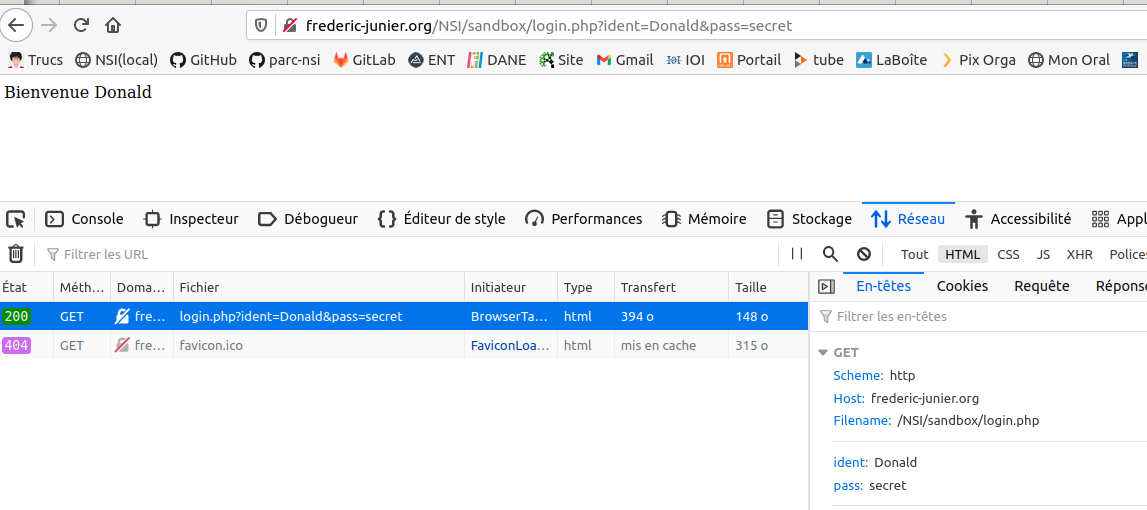
\includegraphics{images/login_get.png}\\
\end{quote}

\begin{itemize}
\tightlist
\item
  Revenir sur la page du formulaire, ouvrir la fenêtre des outils de
  développement avec \passthrough{\lstinline!F12!} et modifier le code
  source pour que l'envoi du mot de passe soit sécurisé.
\end{itemize}

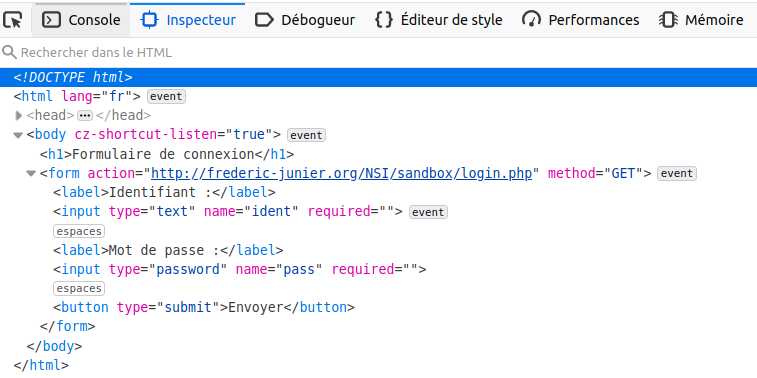
\includegraphics[width=0.6\textwidth,height=\textheight]{images/login.png}\\

\begin{quote}
\emph{Réponse : on effectue deux modifications dans le code source du
formulaire : on utilise la méthode \href{POST}{PSOT} et on passe en
\url{HTTPS} le protocole de l'\url{URL} cible}
\end{quote}

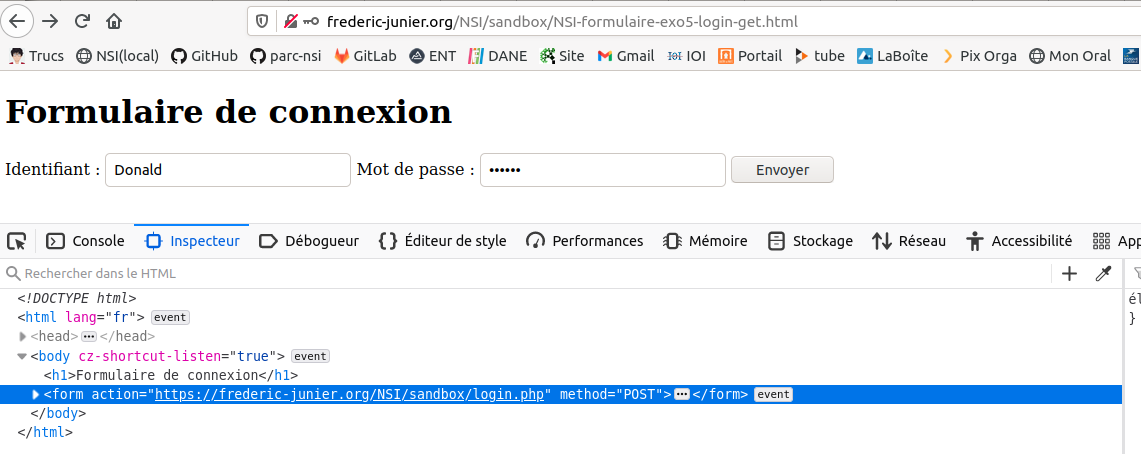
\includegraphics{images/login_https.png}\\

\begin{itemize}
\tightlist
\item
  Dans le schéma ci-dessous d'un échange Web sécurisé avec le protocole
  \href{https://developer.mozilla.org/fr/docs/Glossaire/https}{HTTPS},
  apparaît la notion de
  \href{https://developer.mozilla.org/fr/docs/Glossaire/Certificat_num\%C3\%A9rique}{certificat}.
  Quel est le rôle d'un
  \href{https://developer.mozilla.org/fr/docs/Glossaire/Certificat_num\%C3\%A9rique}{certificat}
  et comment est-il géré par le navigateur ?
\end{itemize}

\begin{quote}
\emph{Réponse : lire la BD ci-dessous et consulter cette page
\url{https://support.mozilla.org/fr/kb/certificats-authentification-pour-sites-web-securises}}
\end{quote}

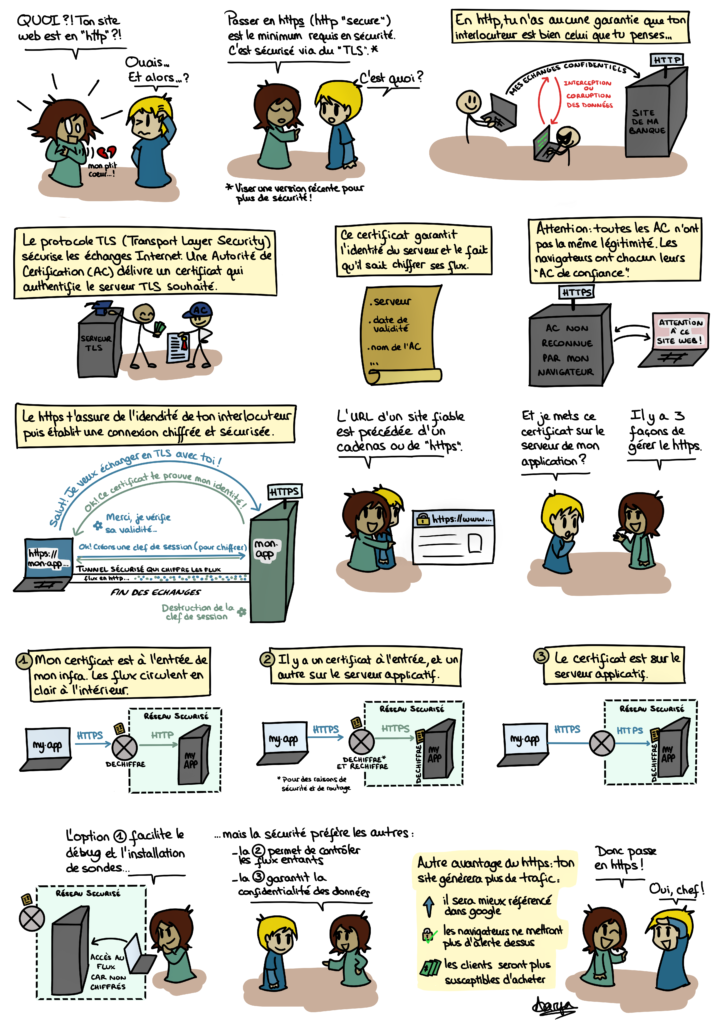
\includegraphics[width=0.87\textwidth,height=\textheight]{images/tls-3-717x1024.png}\\

\emph{Source : \url{https://blog.octo.com/bd-le-https/}}

\end{exercice}

\end{document}
